\documentclass[aspectratio=169, usenames, dvipsnames]{beamer}

%%%%%
%%%%%
%%%%%     DEFINE THE THEME USED
%%%%%
%%%%%

\usetheme{jc}


%%%%%%%%%%%%%%%%%%%%%%%%%%%%%%%%%%%%%%%%%%%%%%%%%
%%%%%                                       %%%%%
%%%%%     LIST OF USEFUL LaTeX PACKAGES     %%%%%
%%%%%                                       %%%%%
%%%%%%%%%%%%%%%%%%%%%%%%%%%%%%%%%%%%%%%%%%%%%%%%%

% ---
% Character encoding
% ---
\usepackage[T1]{fontenc}
\usepackage[utf8]{inputenc}

% ---
% Language related packages
% ---
\usepackage[english]{babel}
\usepackage[abbreviations,british]{foreign}

% ---
% Bibliography-related
% ---
\usepackage[numbers, sort&compress]{natbib}

% ---
% Colours
% ---
\usepackage[]{color}
\usepackage[]{xcolor}

% ---
% Figures
% ---
\usepackage[]{graphicx}
\usepackage[]{subfigure}

% ---
% Mathematics
% ---
\usepackage[]{mathtools}
\usepackage[]{amssymb, amsmath, amsfonts}
\usepackage[]{yhmath}
\usepackage[]{stmaryrd}
\usepackage[]{nicefrac}
\usepackage[]{algpseudocode}

% ---
% Physics
% ---
\usepackage[]{siunitx}
\usepackage[]{physics}

% ---
% In-text references
% ---
\usepackage[]{hyperref}
\usepackage[noabbrev]{cleveref}

% ---
% Typography-related
% ---
\usepackage[protrusion=true,activate={true,nocompatibility},final,tracking=true,kerning=true,spacing=true,factor=1100]{microtype}

\clubpenalty         = 10000
\widowpenalty        = 10000
\displaywidowpenalty = 10000

% ---
% Tikz-related
% ---
\usepackage[]{tikz}
\usetikzlibrary{arrows}
\usetikzlibrary{shapes}
\usetikzlibrary{positioning}
\usetikzlibrary{tikzmark}
\usetikzlibrary{patterns}
\usetikzlibrary{backgrounds}

% ---
% Miscellaneous
% ---
\usepackage[]{lipsum}
\usepackage[]{xparse}

%%%%%%%%%%%%%%%%%%%%%%%%%%%%%%%%%%%%%%%%%%%%%%%
%%%%%                                     %%%%%
%%%%%     LIST OF COMMANDS AND MACROS     %%%%%
%%%%%                                     %%%%%
%%%%%%%%%%%%%%%%%%%%%%%%%%%%%%%%%%%%%%%%%%%%%%%

% ---
% Annotating equations using Tikz
% ---
\newcommand{\highlight}[2]{\colorbox{#1!17}{\ensuremath{\displaystyle #2}}}
\newcommand{\highlightdark}[2]{\colorbox{#1!47}{\ensuremath{\displaystyle #2}}}

% ---
% Mathematics
% ---

% Simple macros
\renewcommand{\det}[1]{\text{det}\left( #1 \right)}
\renewcommand{\trace}[1]{\text{Tr}\left( #1 \right)}
\newcommand{\Span}[1]{\text{Span}\left( #1 \right)}
\newcommand{\conj}[1]{\ensuremath{#1^*}}


% Algebra
\newcommand{\e}{\ensuremath{\mathrm{e}}}

\newcommand{\R}{\ensuremath{\mathbb{R}}}
\newcommand{\C}{\ensuremath{\mathbb{C}}}
\newcommand{\K}{\ensuremath{\mathbb{K}}}

\newcommand{\innerprod}[2]{\ensuremath{\left\langle #1 \vert #2 \right\rangle}}

% Linear algebra
\newcommand{\allones}{\ensuremath{\mathbf{1}}}
\newcommand{\allzeros}{\ensuremath{\mathbf{0}}}
\newcommand{\Gram}[1]{\ensuremath{\mathbf{#1}^H \mathbf{#1}}}
\newcommand{\inv}[1]{\ensuremath{\mathbf{#1}^{-1}}}
\newcommand{\pinv}[1]{\ensuremath{\mathbf{#1}^{\dagger}}}
\newcommand{\svd}[1]{\ensuremath{\mathbf{U}_{#1} \boldsymbol{\Sigma}_{#1} \mathbf{V}^H_{#1}}}

% Probability and statistics
\newcommand{\E}[1]{\ensuremath{\mathbb{E} \left( #1 \right)}}
\newcommand{\covmat}[1]{\ensuremath{\mathbf{C}_{\mathbf{#1}}}}

% Optimization problems
\DeclareMathOperator*{\minimize}{minimize~}
\DeclareMathOperator*{\argmin}{argmin~}

\DeclareMathOperator*{\maximize}{maximize~}
\DeclareMathOperator*{\argmax}{argmax~}

\DeclareMathOperator{\subto}{subject~to~}

% Column and row vectors.
\ExplSyntaxOn
\NewDocumentCommand{\colvec}{O{1}m}
{
  \scalebox{#1}{$\generalvec{#2}{\\}$}
}
\NewDocumentCommand{\rowvec}{O{1}m}
{
  \scalebox{#1}{$\generalvec{#2}{&}$}
}
\NewDocumentCommand{\generalvec}{mm}
{
  \clist_set:Nn \l_tmpa_clist { #1 }
  %\renewcommand{\arraystretch}{.8}
  \begin{bmatrix}
    \clist_use:Nn \l_tmpa_clist { #2 }
  \end{bmatrix}
}
\ExplSyntaxOff
\usefonttheme{professionalfonts}

\graphicspath{{./imgs/}}

%%%%%
%%%%%
%%%%%     INFO ABOUT THE PRESENTATION
%%%%%
%%%%%

\title{Time-stepping approach to \\ large-scale linear algebra}
\author[JC]{Jean-Christophe Loiseau}
%\date[]{November, 17\textsuperscript{th} 2022}

%%%%%
%%%%%
%%%%%     PRESENTATION
%%%%%
%%%%%

\begin{document}

\begin{frame}
  \titlepage
\end{frame}

\begin{frame}
  \vfill
  \begin{minipage}{.32\textwidth}
    \centering
    
\includegraphics[height=.42\textheight]{ricardo}
  \end{minipage}%
  \hfill
  \begin{minipage}{.32\textwidth}
    \centering
    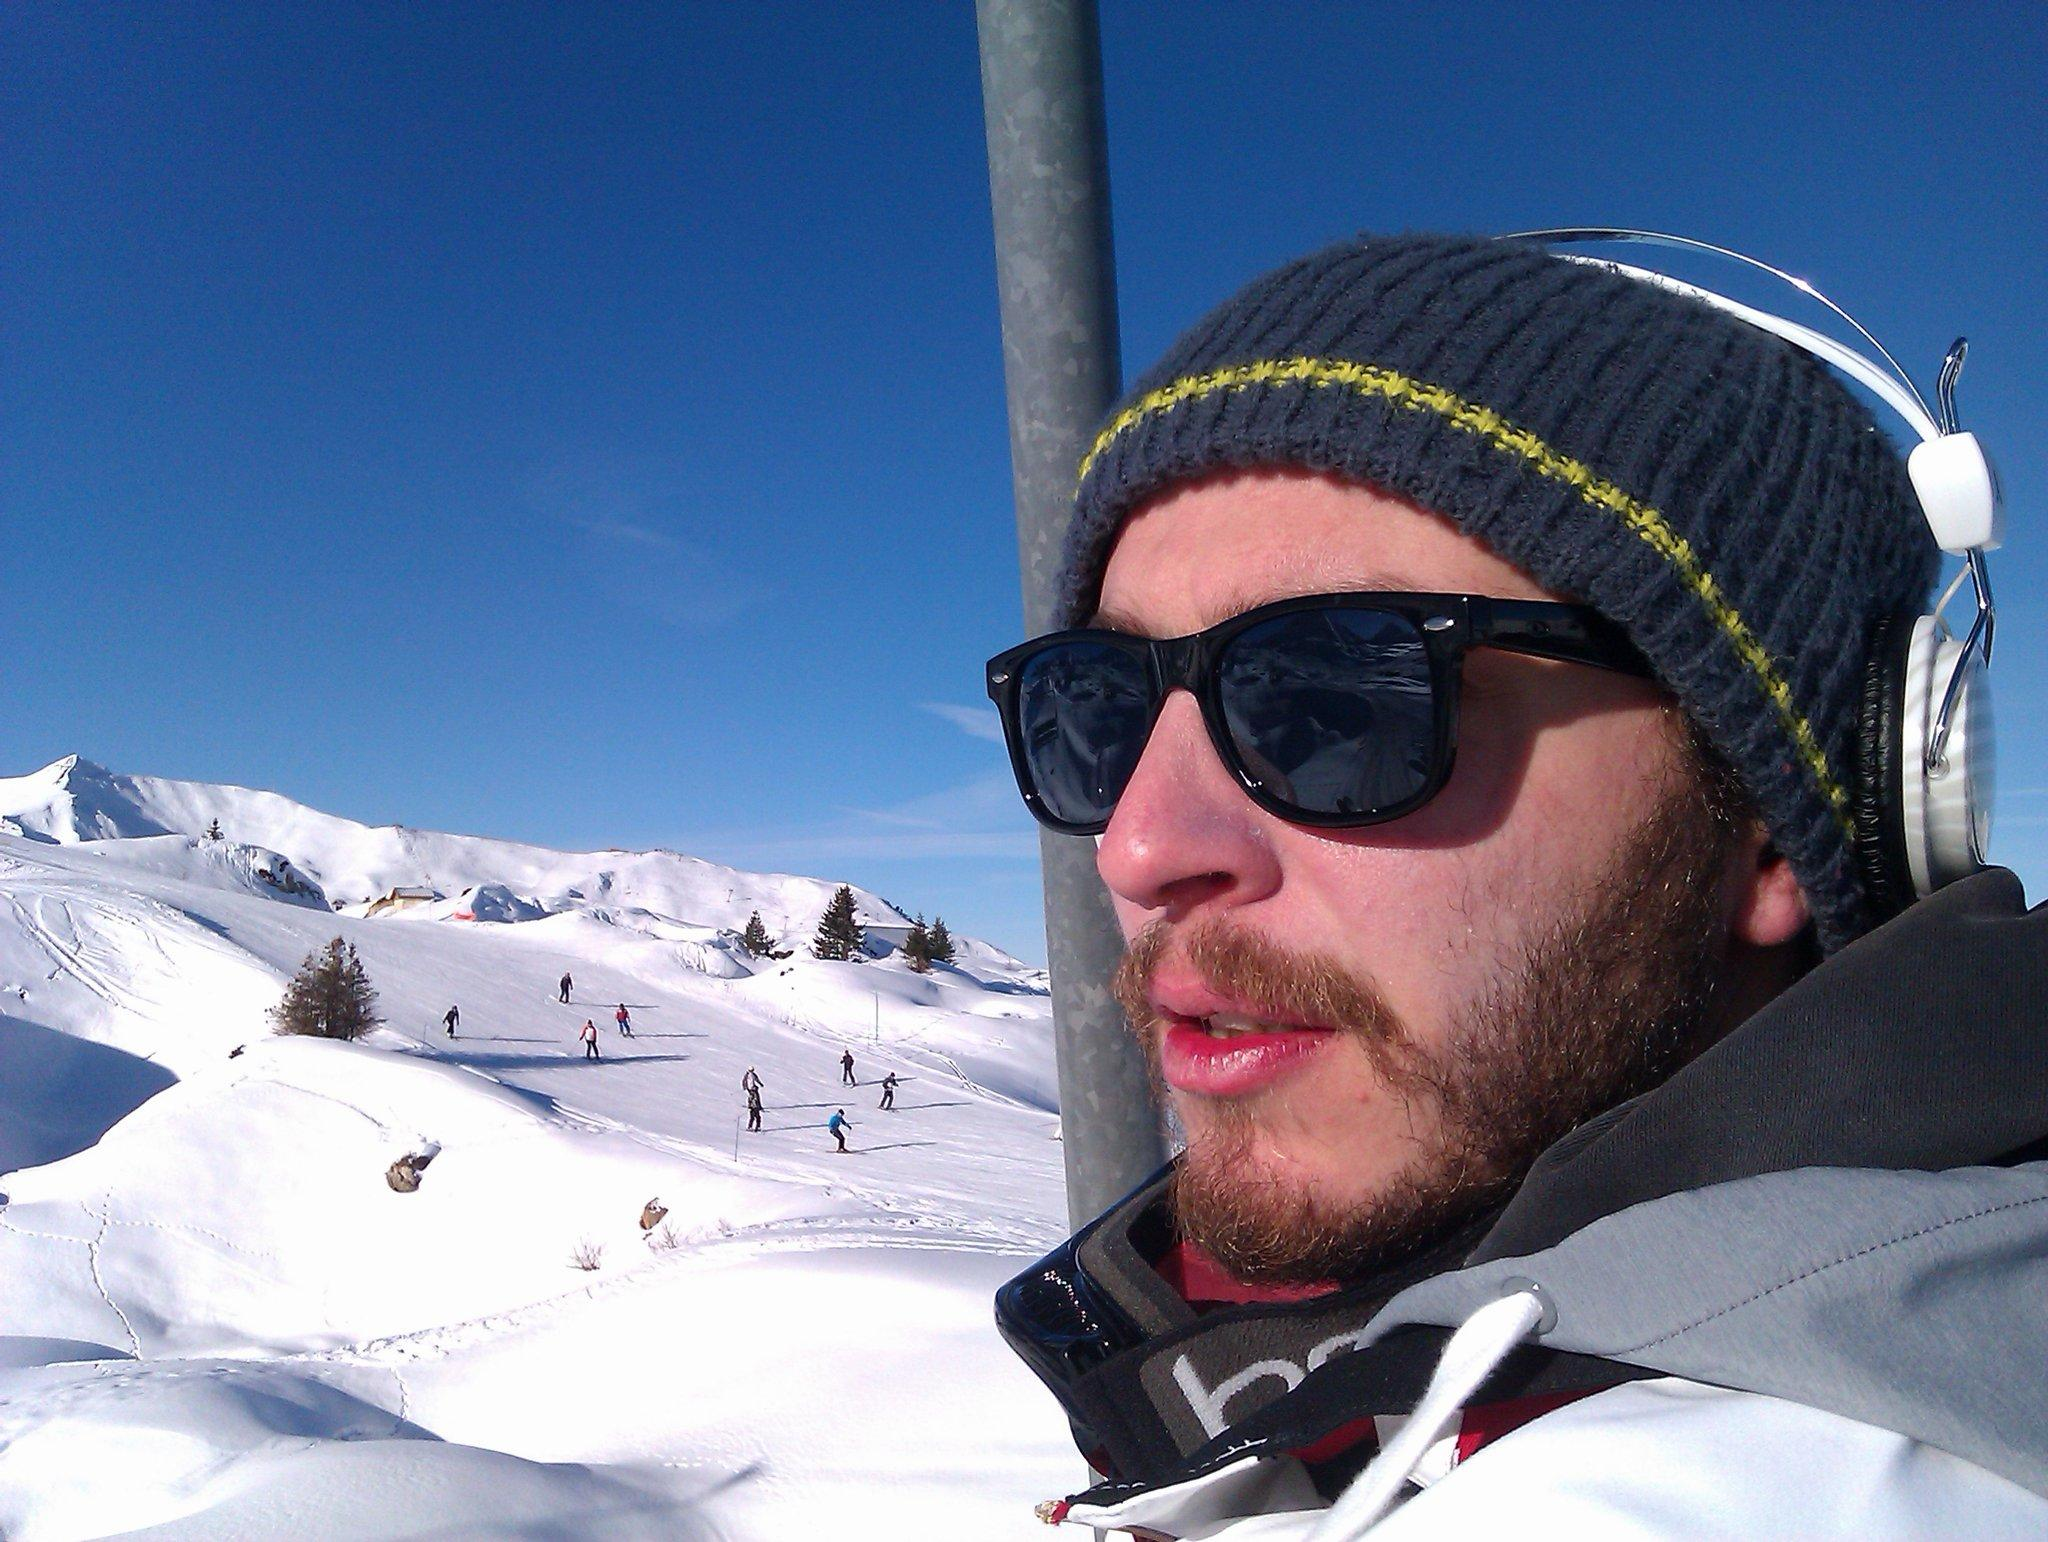
\includegraphics[height=.42\textheight]{myself}
  \end{minipage}
  %
  \hfill
  \begin{minipage}{.32\textwidth}
    \centering
    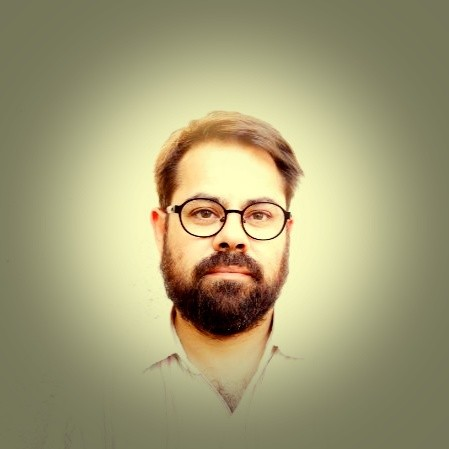
\includegraphics[height=.42\textheight]{robinet}
  \end{minipage}

  \bigskip
  \begin{minipage}{.32\textwidth}
    \centering
    \tiny
    Ricardo Frantz
  \end{minipage}%
  \hfill
  \begin{minipage}{.32\textwidth}
    \centering
    \tiny
    Jean-Christophe Loiseau
  \end{minipage}
  %
  \hfill
  \begin{minipage}{.32\textwidth}
    \centering
    \tiny
    Jean-Christophe Robinet
  \end{minipage}

  \vfill
\end{frame}




%%%%%%%%%%%%%%%%%%%%%%%%%%%%%%%%
%%%%%                      %%%%%
%%%%%     INTRODUCTION     %%%%%
%%%%%                      %%%%%
%%%%%%%%%%%%%%%%%%%%%%%%%%%%%%%%

\begin{frame}
  \vfill
  \begin{minipage}{.40\textwidth}
    \centering
    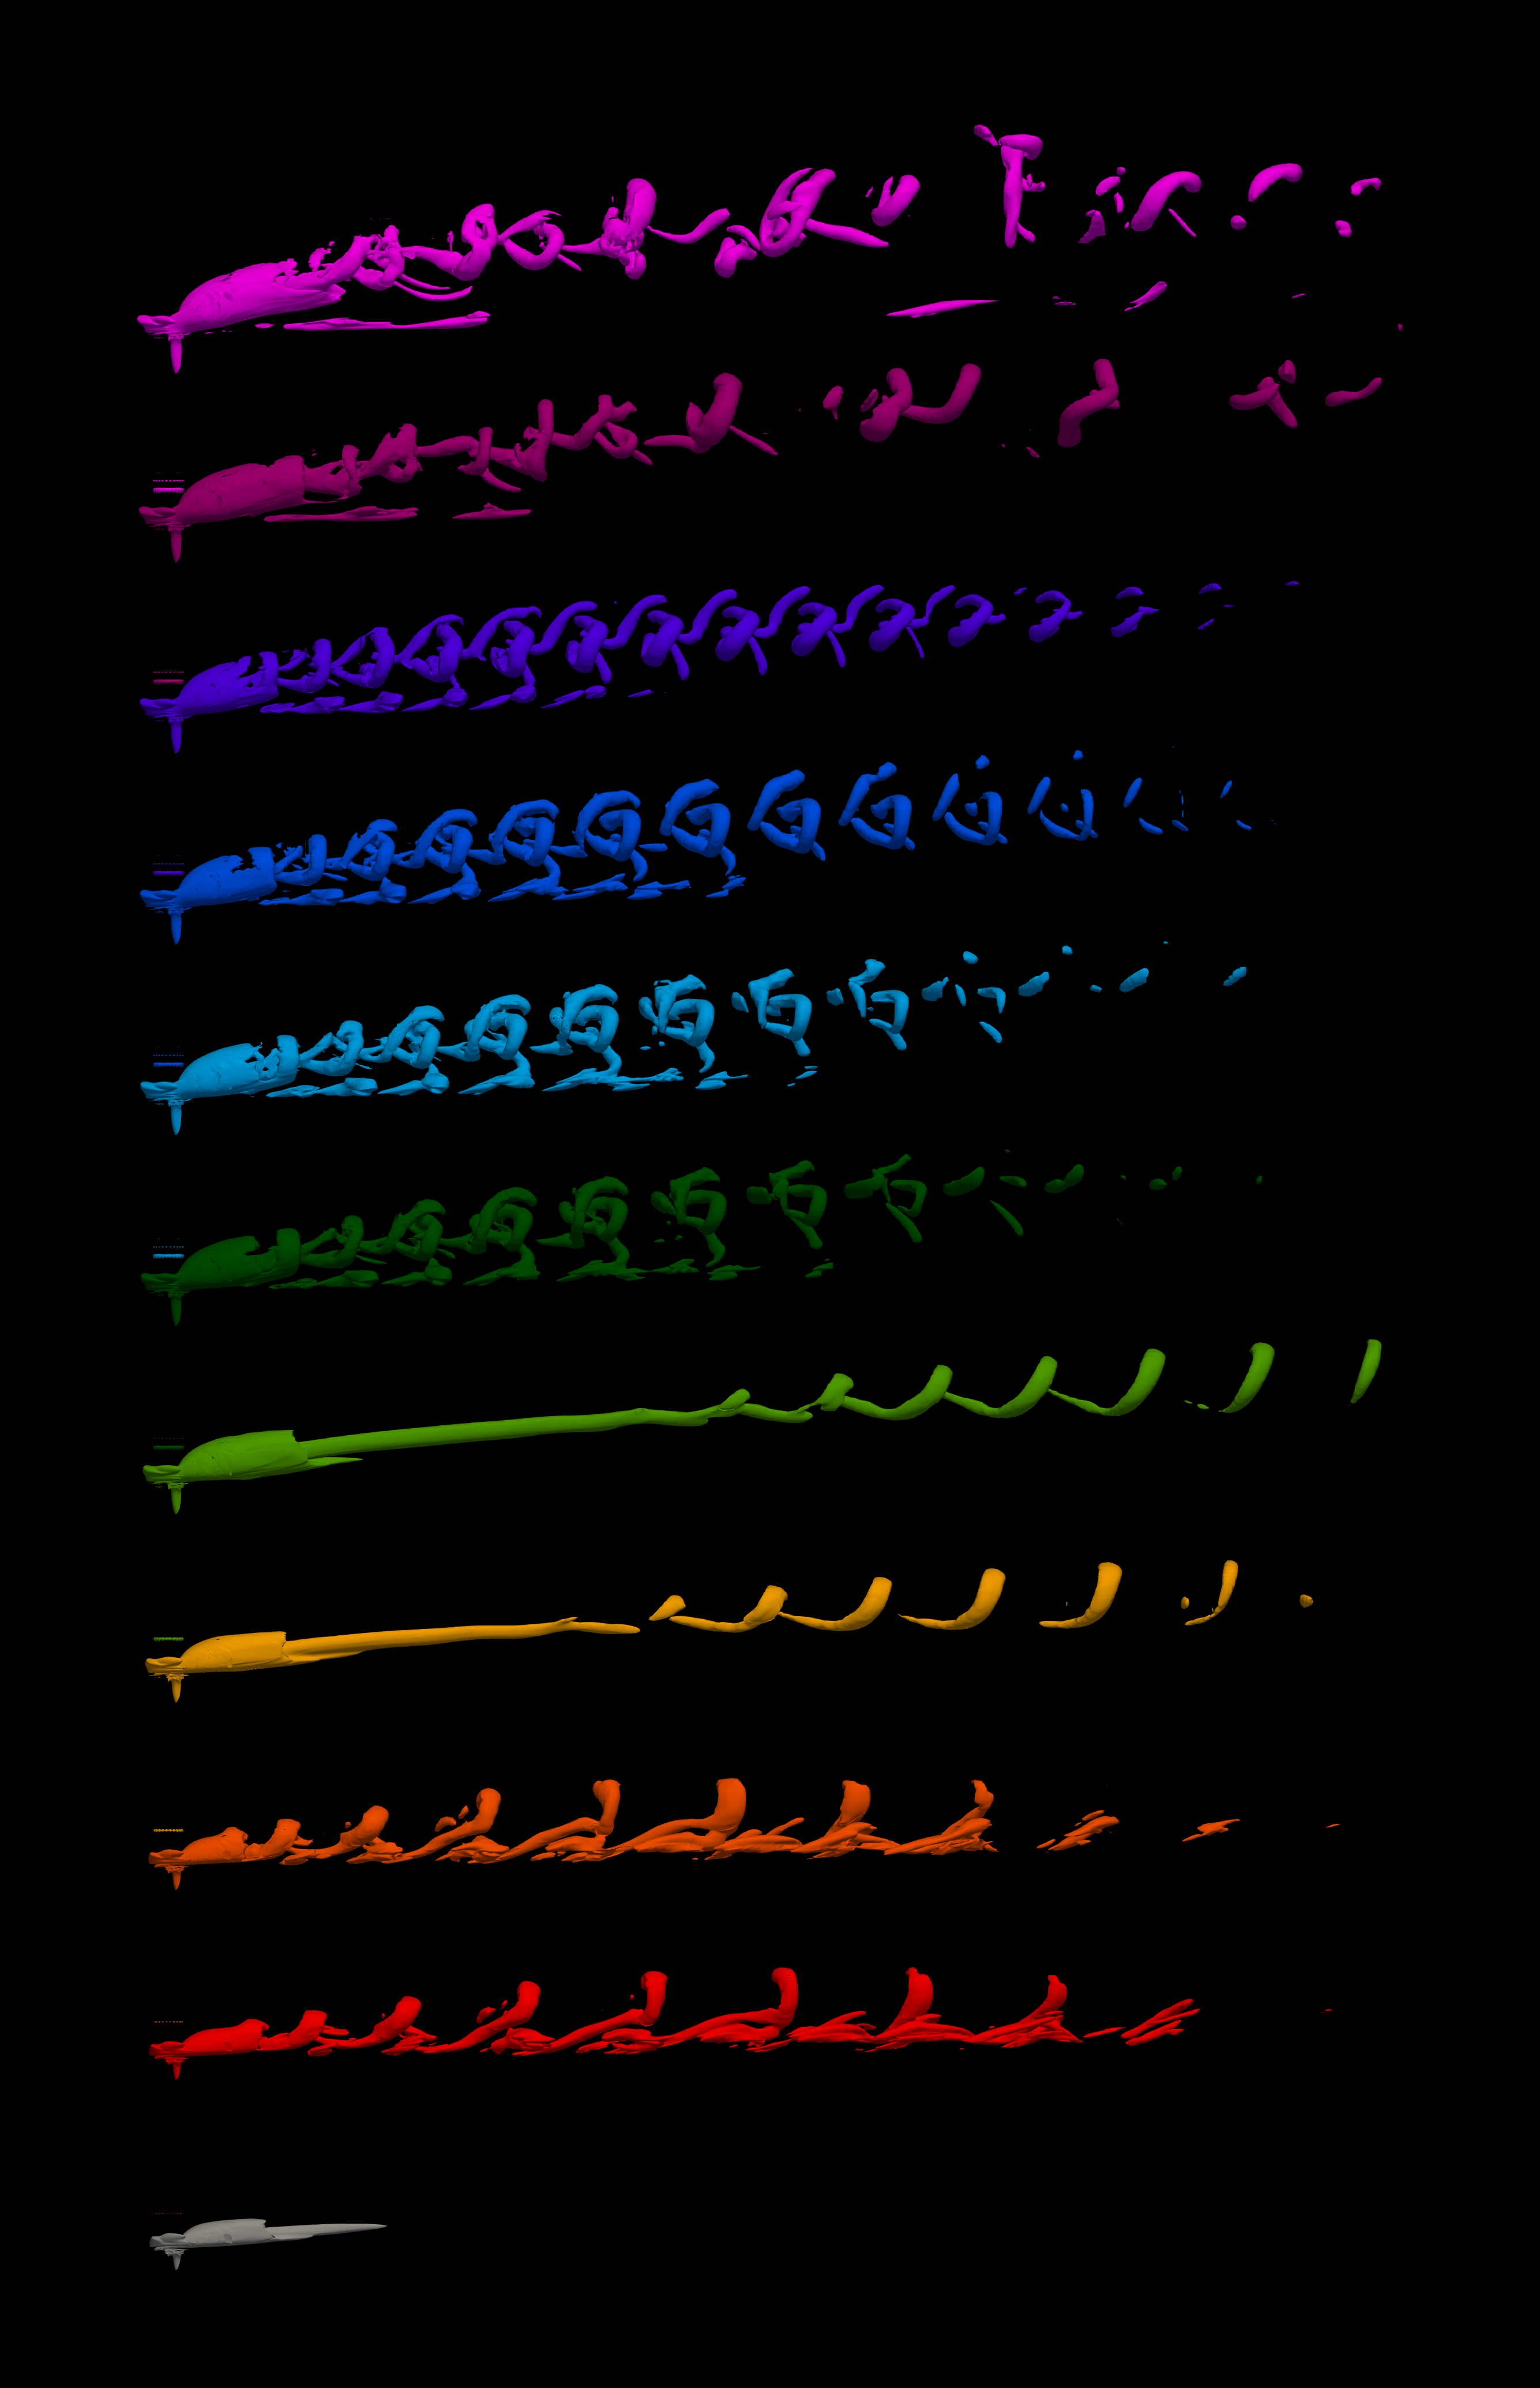
\includegraphics[width=\textwidth]{jet_in_xflow}
  \end{minipage}%
  \hfill
  \begin{minipage}{.56\textwidth}
    \textbf{Hydrodynamic stability :} Set of tools to investigate the first stages of transition to turbulence.
    
    \bigskip
    
    Primarily a numerical linear algebra issue for large-scale dynamical systems such as discretized PDEs.
  \end{minipage}
  \vfill
\end{frame}

{
  \setbeamercolor*{background canvas}{bg=white}
  \setbeamercolor{normal text}{fg=black}
  \usebeamercolor[fg]{normal text}
  \setbeamercolor{item}{fg=black}

  \begin{frame}
    \vfill
    \includegraphics[width=\textwidth]{fig9}
    \vfill
  \end{frame}
}  
  
\begin{frame}
  \vfill

  {
    \Large
    \[
      \dot{\vb{X}} = \tikzmarknode{a}{\highlightdark{red}{f}} \left( t, \tikzmarknode{b}{\highlightdark{blue}{\vb{X}}}, \boldsymbol{\mu} \right)
    \]
  }
  \begin{tikzpicture}[overlay, remember picture, >=stealth, nodes={align=left, inner ysep=1pt}, <-]
    \path (a.north) ++ (0, 2em) node[anchor=south east, color=red!67] (dynamics){Dynamics $f : \R \times \R^n \times \R^p \to \R^n$};
    \draw [color=red!87] (a.north) |- ([xshift=0.3ex, color=red] dynamics.south west);

    \path (b.south) ++ (0, -2em) node[anchor=north west, color=blue!67] (state){State vector $\vb{X} \in \R^n$};
    \draw [color=blue!87] (b.south) |- ([xshift=0.3ex, color=blue] state.south east);
  \end{tikzpicture}
  \vfill
\end{frame}

\begin{frame}
  \vfill
  {
    \Large
    \[
      \vb{X}_{k+1} = \tikzmarknode{a}{\highlightdark{red}{\varphi_{\tau}}} \left( \vb{X}_k, \boldsymbol{\mu} \right)
    \]
  }
  \begin{tikzpicture}[overlay, remember picture, >=stealth, nodes={align=left, inner ysep=1pt}, <-]
    \path (a.north) ++ (0, 2em) node[anchor=south east, color=red!67] (dynamics){Flow map $\varphi_\tau : \R^n \times \R^p \to \R^n$};
    \draw [color=red!87] (a.north) |- ([xshift=0.3ex, color=red] dynamics.south west);
  \end{tikzpicture}
 
  \vfill
\end{frame}

\begin{frame}
  \vfill

  \centering

  \textbf{
    How to compute fixed points or periodic orbits of the system and study their linear stability properties given only a time-stepper ?
  }
  
  \vfill
\end{frame}

\begin{frame}
  \vfill
  \centering
  \underline{\textbf{Fixed points}}

  \vfill
  
  \begin{minipage}{.48\textwidth}
    \centering
    \emph{Continuous time}
    {
      \Large
      \[
        f(\vb{X}, \boldsymbol{\mu}) = \allzeros
      \]
    }
  \end{minipage}%
  \hfill
  \begin{minipage}{.48\textwidth}
    \centering
    \emph{Discrete time}
    {
      \Large
      \[
        \varphi_{\tau}(\vb{X}, \boldsymbol{\mu}) - \vb{X}= \allzeros \quad \forall \tau
      \]
    }
  \end{minipage}
  \vfill
\end{frame}

\begin{frame}
  \vfill
  \centering
  \underline{\textbf{Linearized system}}

  \vfill

  \begin{minipage}{.48\textwidth}
    \centering
    \emph{Continuous time}
    {
      \Large
      \[
        \dot{\vb{x}} = \tikzmarknode{a}{\highlightdark{red}{\vb{L}}} \vb{x}
      \]
    }
    \begin{tikzpicture}[overlay, remember picture, >=stealth, nodes={align=left, inner ysep=1pt}, <-]
      \path (a.south) ++ (0, -2em) node[anchor=south east, color=red!67] (dynamics){Jacobian matrix $\in \R^{n \times n}$};
      \draw [color=red!87] (a.south) |- ([xshift=0.3ex, color=red] dynamics.south west);
    \end{tikzpicture}
  \end{minipage}%
  \hfill
  \begin{minipage}{.48\textwidth}
    \centering
    \emph{Discrete time}
    {
      \Large
      \[
        \vb{x}_{k+1} = \tikzmarknode{b}{\highlightdark{blue}{\exp(\tau \vb{L})}} \vb{x}_k
      \]
    }
    \begin{tikzpicture}[overlay, remember picture, >=stealth, nodes={align=left, inner ysep=1pt}, <-]
      \path (b.south) ++ (0, -2em) node[anchor=south east, color=blue!67] (dynamics){Exponential Propagator $\in \R^{n \times n}$};
      \draw [color=blue!87] (b.south) |- ([xshift=0.3ex, color=blue] dynamics.south west);
    \end{tikzpicture}
  \end{minipage}
  
  \vfill
\end{frame}

\begin{frame}
  \vfill
  \centering
  \underline{\textbf{Arnoldi factorization}}

  \vfill

  \begin{minipage}{.48\textwidth}
    \centering
    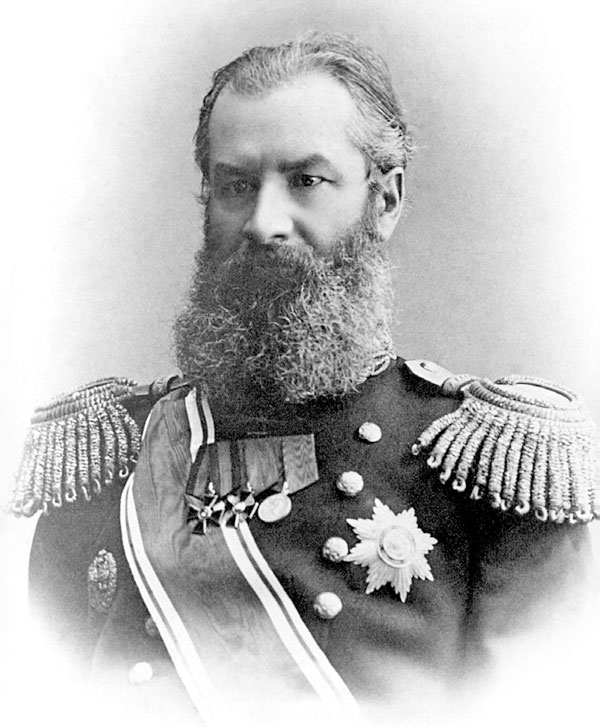
\includegraphics[width=.5\textwidth]{krylov}

    {\tiny
      Alexei Krylov
    }
  \end{minipage}%
  \hfill
  \begin{minipage}{.48\textwidth}
    \centering
    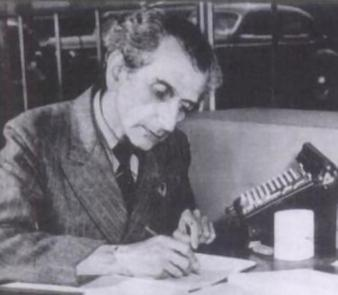
\includegraphics[width=.7\textwidth]{lanczos}

    {\tiny
      Cornelius Lanczos
    }
  \end{minipage}
  
  \vfill
\end{frame}

\begin{frame}
  \vfill
  \centering

  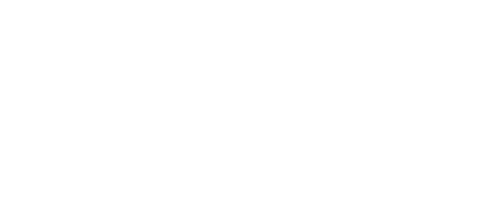
\includegraphics[width=.8\textwidth]{arnoldi}
  
  \vfill
\end{frame}

\begin{frame}
  \vfill
  \centering
  \underline{\textbf{Generalized Minimal Residual Method}}

  \vfill

  \begin{minipage}{.48\textwidth}
    \begin{algorithmic}
      \Require $\vb{x}_0$, $\vb{A}$, $\vb{b}$
      \Ensure $\norm{\vb{Ax} - \vb{b}}_2^2 \leq \varepsilon$
      \State $\vb{r} \gets \vb{b} - \vb{Ax}_0$
      \State $\vb{q}_1 \gets \vb{r} / \norm{\vb{r}}_2$
      \For{$k = 1, 2, \cdots$}
      \State $\vb{y} \gets \vb{Aq}_k$
      \For{$j = 1, 2, \cdots, k$}
      \State $h_{jk} \gets \vb{q}^T_j \vb{y}$
      \State $\vb{y} \gets \vb{y} - h_{jk} \vb{q}_j$
      \EndFor
      \State $h{k+1, k} = \norm{\vb{y}}_2$
      \State $\vb{q}_{k+1} = \vb{y} / h_{k+1, k}$
      \State $\minimize~\norm{\vb{Hc} - \vb{e}_1 \norm{\vb{r}}_2}_2$
      \State $\vb{x}_k \gets \vb{x}_0 + \vb{Q}_k \vb{c}$
      \EndFor
    \end{algorithmic}
  \end{minipage}%
  \hfill
  \begin{minipage}{.48\textwidth}
    \centering
    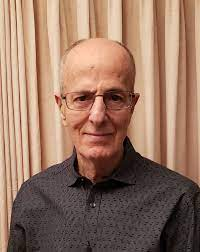
\includegraphics[width=.6\textwidth]{saad}

    {\tiny
      Youssef Saad
    }
  \end{minipage}
  
  \vfill
\end{frame}

\begin{frame}
  \vfill
  \begin{minipage}{.48\textwidth}
    \centering
    {
      \huge
      \textbf{Fixed point computation}
    }
  \end{minipage}%
  \hfill
  \begin{minipage}{.48\textwidth}
  \end{minipage}

  \vfill
\end{frame}

\begin{frame}
  \vfill

  {
    \Large
    \[
      \mathcal{F}(\vb{X}, \boldsymbol{\mu}) \equiv \varphi_{\tau}\left( \vb{X}, \boldsymbol{\mu} \right) - \vb{X} = \allzeros
    \]
  }
  
  \vfill
\end{frame}

\begin{frame}
  \vfill

  {
    \Large
    \[
      \vb{J} \equiv \exp \left( \tau \vb{L} \right) - \vb{I}
    \]
  }
  \vfill
\end{frame}

\begin{frame}
  \vfill
  \centering
  \textbf{Newton-GMRES solver for fixed point computation}

  \vfill
  
  \begin{minipage}{.48\textwidth}
    \begin{algorithmic}
      \Require $\vb{X}$
      \Ensure $\norm{\vb{F}(\vb{X})} \leq \varepsilon$
      \State $\vb{r} \gets \mathcal{F}(\vb{X}_0)$
      \While{ $\norm{\vb{r}} \geq \varepsilon$ }
      \State $\delta\vb{x} \gets \mathrm{gmres}(\vb{F}^{\prime}, \vb{r})$
      \State $\vb{X} \gets \vb{X} + \delta\vb{x}$
      \State $\vb{r} \gets \vb{F}(\vb{X})$
      \EndWhile
    \end{algorithmic}
  \end{minipage}%
  \hfill%
  \vrule%
  \hfill
  \begin{minipage}{.48\textwidth}
    \begin{itemize}
    \item The product $\exp\left( \tau \vb{L} \right) \vb{x}$ can easily be computed with a time-stepper.

      \bigskip

    \item Good performances even without preconditionning!

      \bigskip

    \item Extension to periodic orbits is straightforward.
    \end{itemize}
  \end{minipage}
  \vfill
\end{frame}


{
\setbeamercolor*{background canvas}{bg=white}
\setbeamercolor{normal text}{fg=black}
\usebeamercolor[fg]{normal text}
\setbeamercolor{item}{fg=black}

\begin{frame}
  \vfill
  \begin{minipage}{.28\textwidth}
    \centering
    
\includegraphics[width=.8\textwidth]{akervik}

    \bigskip

    {\small
      Espen \AA{}kervik
    }
  \end{minipage}%
  \hfill
  \begin{minipage}{.68\textwidth}
    \centering
    \textbf{Selective Frequency Damping}

    \vspace{2em}
    
    {
      \Large
      \[
        \begin{aligned}
          \dot{\vb{X}} & = f(t, \vb{X}, \boldsymbol{\mu}) - \tikzmarknode{a}{\highlightdark{red}{\chi}} \left( \vb{X} - \vb{Y} \right) \\
          \dot{\vb{Y}} & = \tikzmarknode{b}{\highlightdark{blue}{\omega_c}} \left(  \vb{X} - \vb{Y} \right)
        \end{aligned}
      \]
    }
    \begin{tikzpicture}[overlay, remember picture, >=stealth, nodes={align=left, inner ysep=1pt}, <-]
      \path (a.north) ++ (0, 2em) node[anchor=south east, color=red!67] (dynamics){Filter's gain};
      \draw [color=red!87] (a.north) |- ([xshift=0.3ex, color=red] dynamics.south west);

      \path (b.south) ++ (0, -2em) node[anchor=north west, color=blue!67] (state){Filter's cutoff frequency};
      \draw [color=blue!87] (b.south) |- ([xshift=0.3ex, color=blue] state.south east);
    \end{tikzpicture}
  \end{minipage}
  \vfill
\end{frame}

\begin{frame}
  \vfill
  \begin{minipage}{.68\textwidth}
    \centering
    \textbf{BoostConv}

    \vspace{2em}
    
    \[
      \tikzmarknode{a}{\highlightdark{red}{\tilde{\vb{x}}_{t+1}}} = \tikzmarknode{b}{\highlightdark{blue}{\vb{x}_{t+1}}} - \vb{YY}^{\dagger}\left( \vb{x}_{t+1} - \tilde{\vb{x}}_t \right) + \vb{XY}^{\dagger} \left( \vb{x}_{t+1} - \tilde{\vb{x}}_t \right)
    \]
    \begin{tikzpicture}[overlay, remember picture, >=stealth, nodes={align=left, inner ysep=1pt}, <-]
      \path (a.north) ++ (0, 2em) node[anchor=south west, color=red!67] (dynamics){Corrected state};
      \draw [color=red!87] (a.north) |- ([xshift=0.3ex, color=red] dynamics.south east);

      \path (b.south) ++ (0, -2em) node[anchor=north west, color=blue!67] (state){Predicted state};
      \draw [color=blue!87] (b.south) |- ([xshift=0.3ex, color=blue] state.south east);
    \end{tikzpicture}
   
  \end{minipage}%
  \hfill
  \begin{minipage}{.28\textwidth}
    \centering
    
\includegraphics[width=\textwidth]{citro}

    \bigskip

    {\small
      Vincenzo Citro
    }
  \end{minipage}
  \vfill
\end{frame}

\begin{frame}
  \vfill
  \vfill
  \begin{minipage}{.28\textwidth}
    \centering
    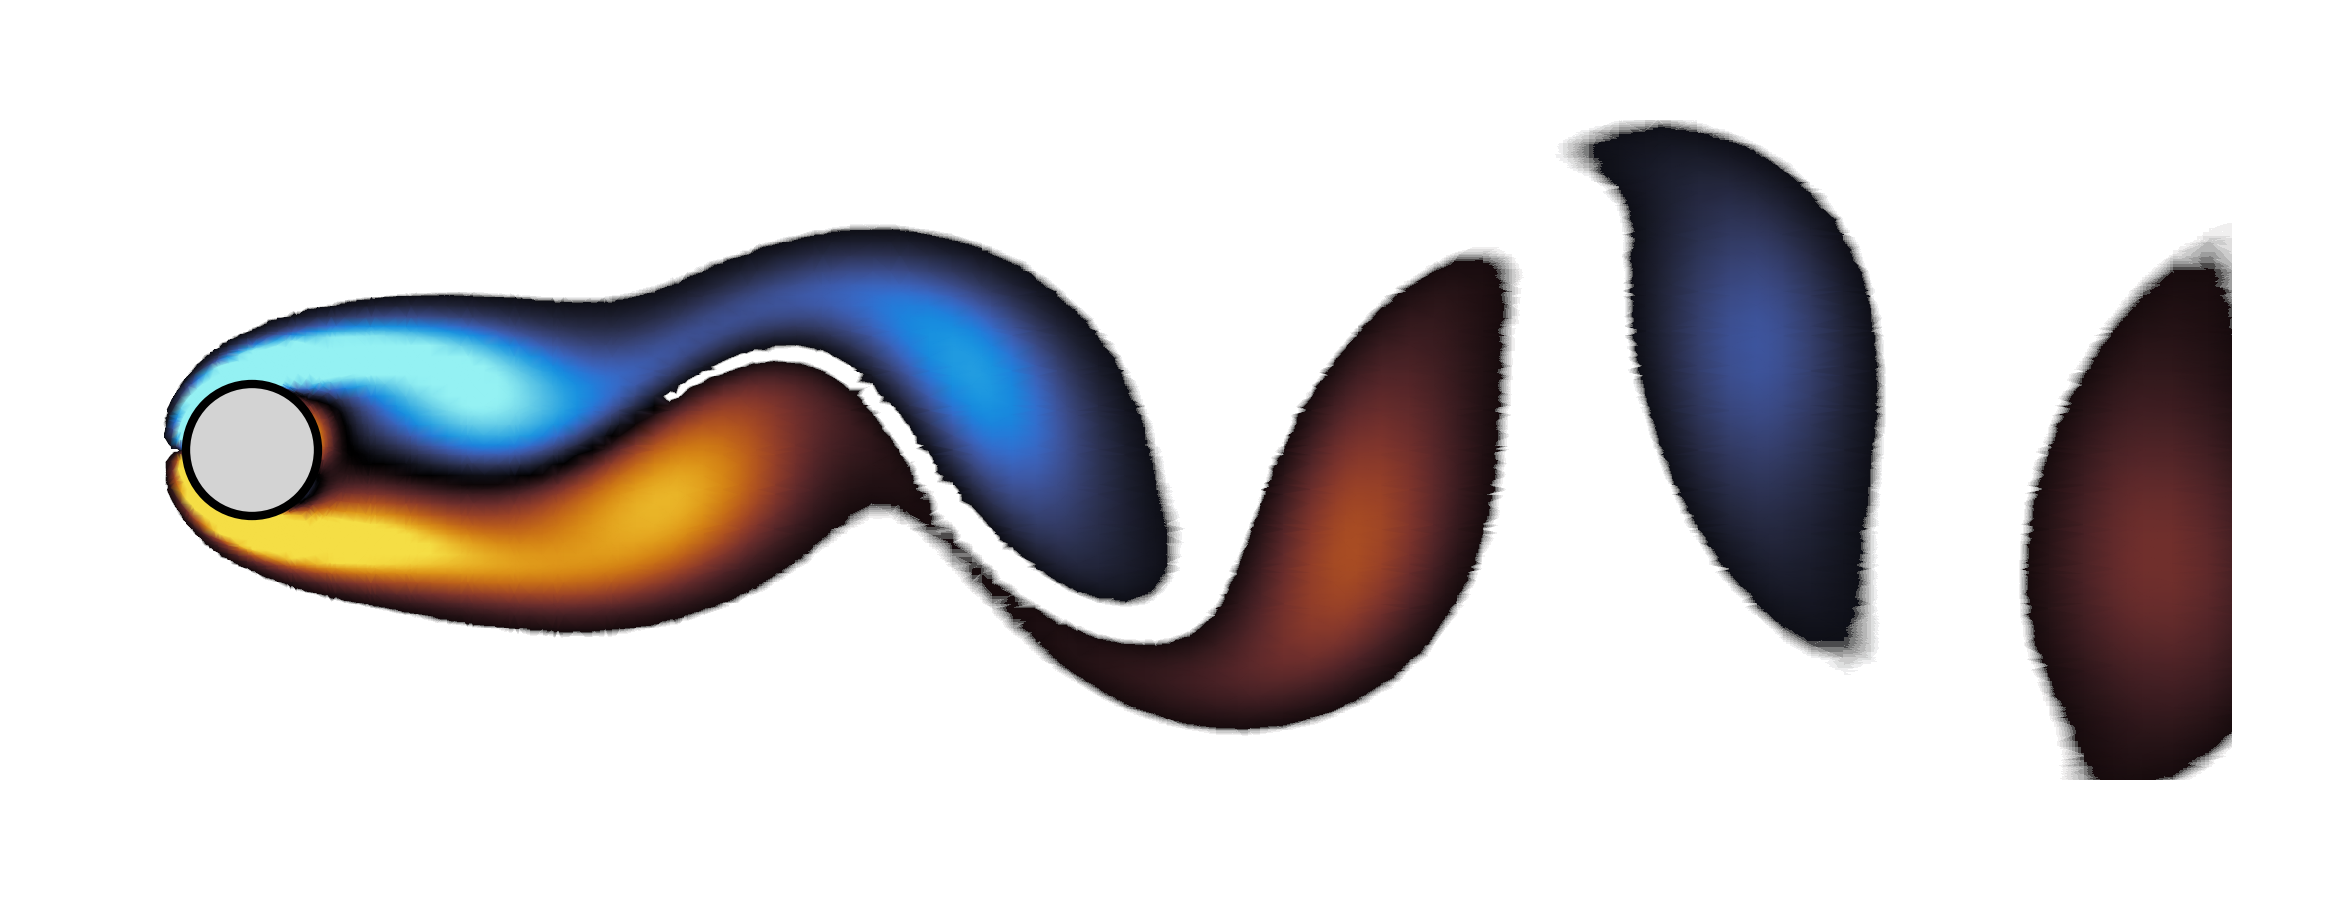
\includegraphics[height=.4\textheight, angle=-90, origin=c]{von_karman_bis}
  \end{minipage}%
  \hfill
  \begin{minipage}{.68\textwidth}
    Standard test case in the incompressible hydrodynamic stability community.
    Here, we solve it with the spectral element solver \texttt{Nek5000} + \texttt{nekStab}.
  \end{minipage}
  \vfill
\end{frame}

\begin{frame}
  \vfill
  \vfill
  \begin{minipage}{.28\textwidth}
    \centering
    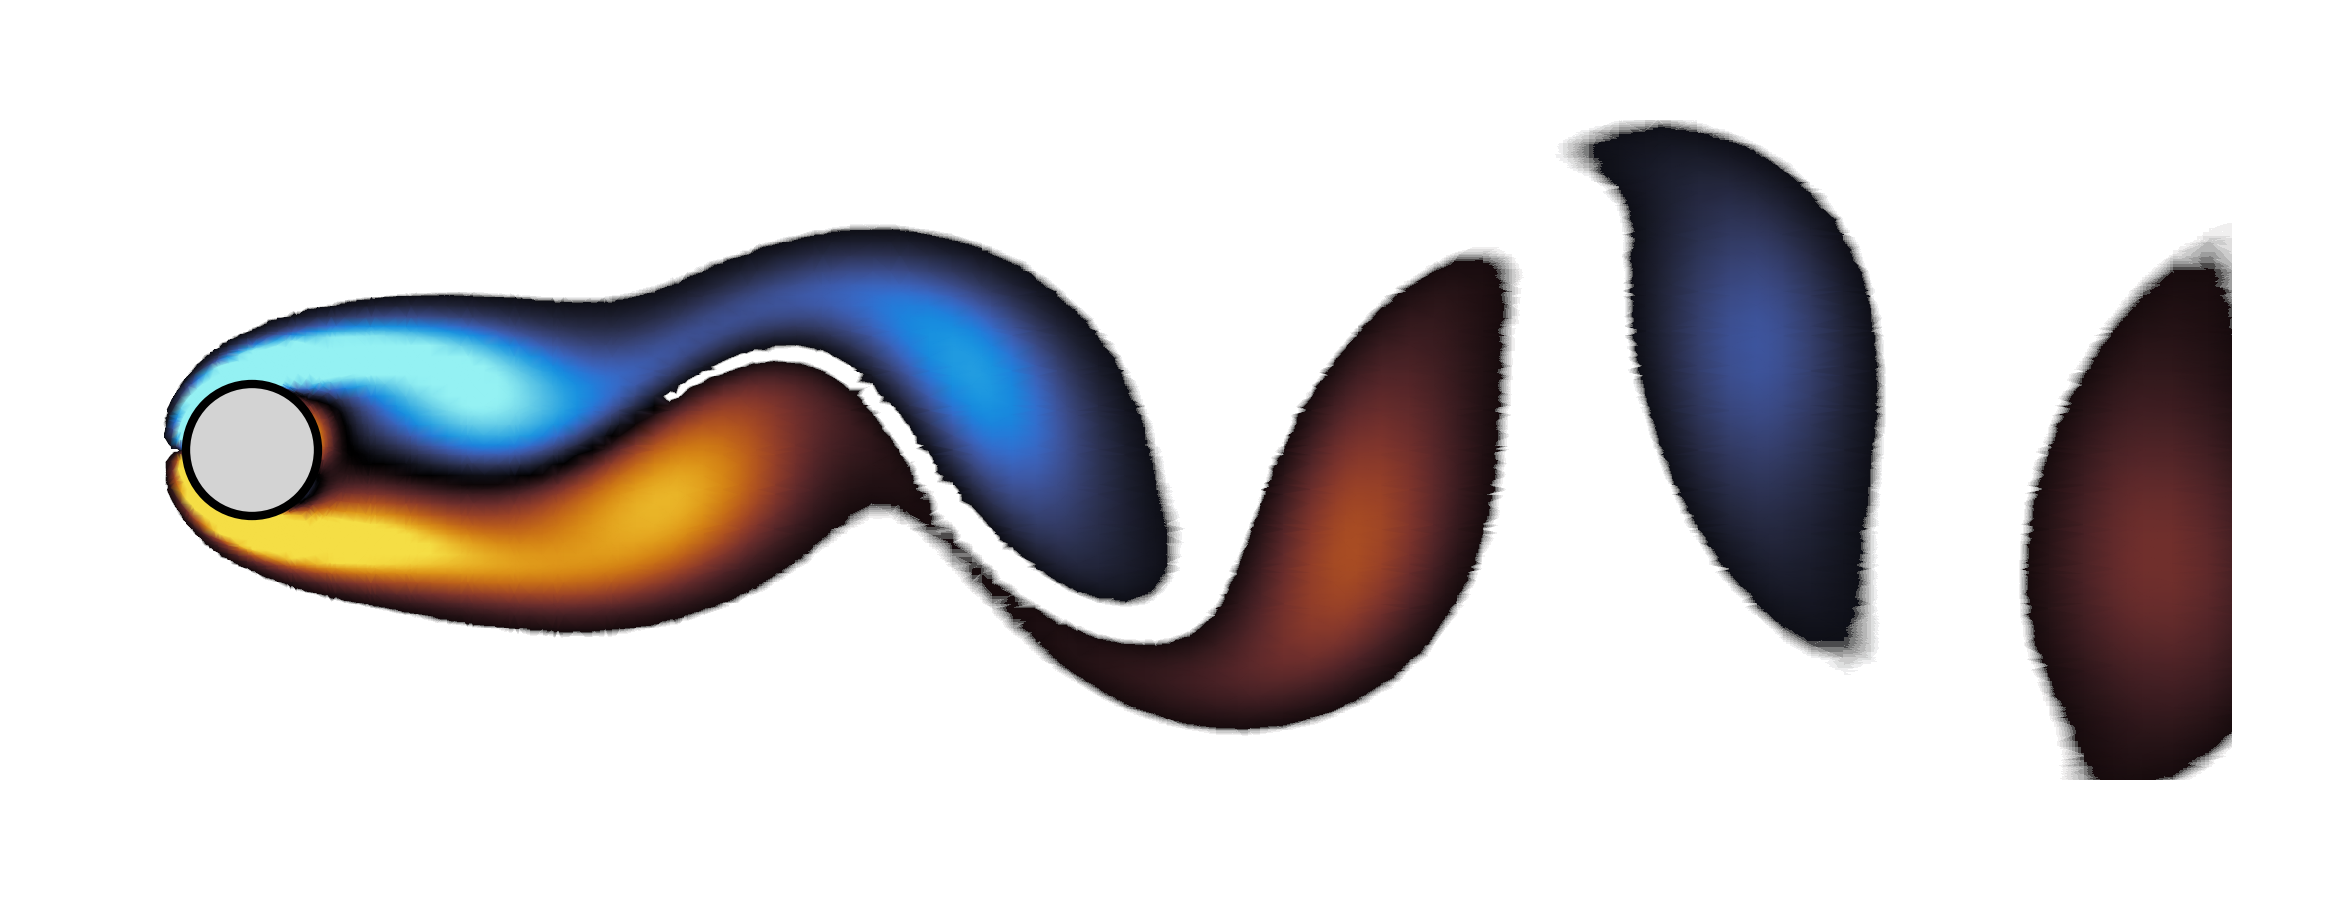
\includegraphics[height=.4\textheight, angle=-90, origin=c]{von_karman_bis}
  \end{minipage}%
  \hfill
  \begin{minipage}{.68\textwidth}
    \begin{itemize}
    \item From $Re = 40 \quad \to \quad Re = 70$.\\
      \medskip
    \item 2000 spectral elements.
      \medskip
    \item 3\textsuperscript{rd} order-accurate EXT/BDF scheme.
      \medskip
    \item Helmholtz solver tolerance set to $10^{-12}$.
      \medskip
    \item Pressure Poisson solver tolerance set to $10^{-10}$.
    \end{itemize}
  \end{minipage}
  \vfill
\end{frame}


\begin{frame}
  \vfill
  \centering
  \textbf{Coarse mesh :} $32\ 000$ grid points with $\Delta t = 0.025$

  \vfill
  
  \begin{tabular}{ccccc}
    ~ & \textbf{SFD} & \textbf{BootConv} & \textbf{Newton-GMRES} & \textbf{Newton-GMRES} (dyn. tol.) \\
    \\
    \hline \\
    \textbf{Time} & 42~\unit{\s} & 30~\unit{\s} & 65~\unit{\s} & 30~\unit{\s}\\
    \\
    \textbf{RAM Usage} & 0.3~\unit{Gb} & 0.4~\unit{Gb} & 1.8~\unit{Gb} & 0.5~\unit{Gb} 
  \end{tabular}
  \vfill
\end{frame}


\begin{frame}
  \vfill
  \centering
  \textbf{Intermediate mesh :} $72\ 000$ grid points with $\Delta t = 0.01$

  \vfill
  
  \begin{tabular}{ccccc}
    ~ & \textbf{SFD} & \textbf{BootConv} & \textbf{Newton-GMRES} & \textbf{Newton-GMRES} (dyn. tol.) \\
    \\
    \hline \\
    \textbf{Time} & 230~\unit{\s} & 235~\unit{\s} & 370~\unit{\s} & 230~\unit{\s}\\
      & ($\times 6$) & ($\times 8$) & ($\times 6$) & ($\times 8$) \\
    \\
    \textbf{RAM Usage} & 0.3~\unit{Gb} & 0.4~\unit{Gb} & 1.8~\unit{Gb} & 0.8~\unit{Gb} 
  \end{tabular}
  \vfill
\end{frame}


\begin{frame}
  \vfill
  \centering
  \textbf{Fine mesh :} $128\ 000$ grid points with $\Delta t = 0.005=$

  \vfill
  
  \begin{tabular}{ccccc}
    ~ & \textbf{SFD} & \textbf{BootConv} & \textbf{Newton-GMRES} & \textbf{Newton-GMRES} (dyn. tol.) \\
    \\
    \hline \\
    \textbf{Time} & 884~\unit{\s} & 1260~\unit{\s} & 1370~\unit{\s} & 774~\unit{\s}\\
      & ($\times 3.8$) & ($\times 5$) & ($\times 3.7$) & ($\times 3.6$) \\
    \\
    \textbf{RAM Usage} & 0.4~\unit{Gb} & 0.6~\unit{Gb} & 2.9~\unit{Gb} & 0.8~\unit{Gb} 
  \end{tabular}
  \vfill
\end{frame}


\begin{frame}
  \vfill
  \begin{minipage}{.68\textwidth}
    Another relatively standard test-case for flow control and reduced-order modeling\footnote{Merci Denis !}.
    A branch of discrete eigenvalues eventually become unstable.
  \end{minipage}%
  \hfill
  \begin{minipage}{.28\textwidth}
    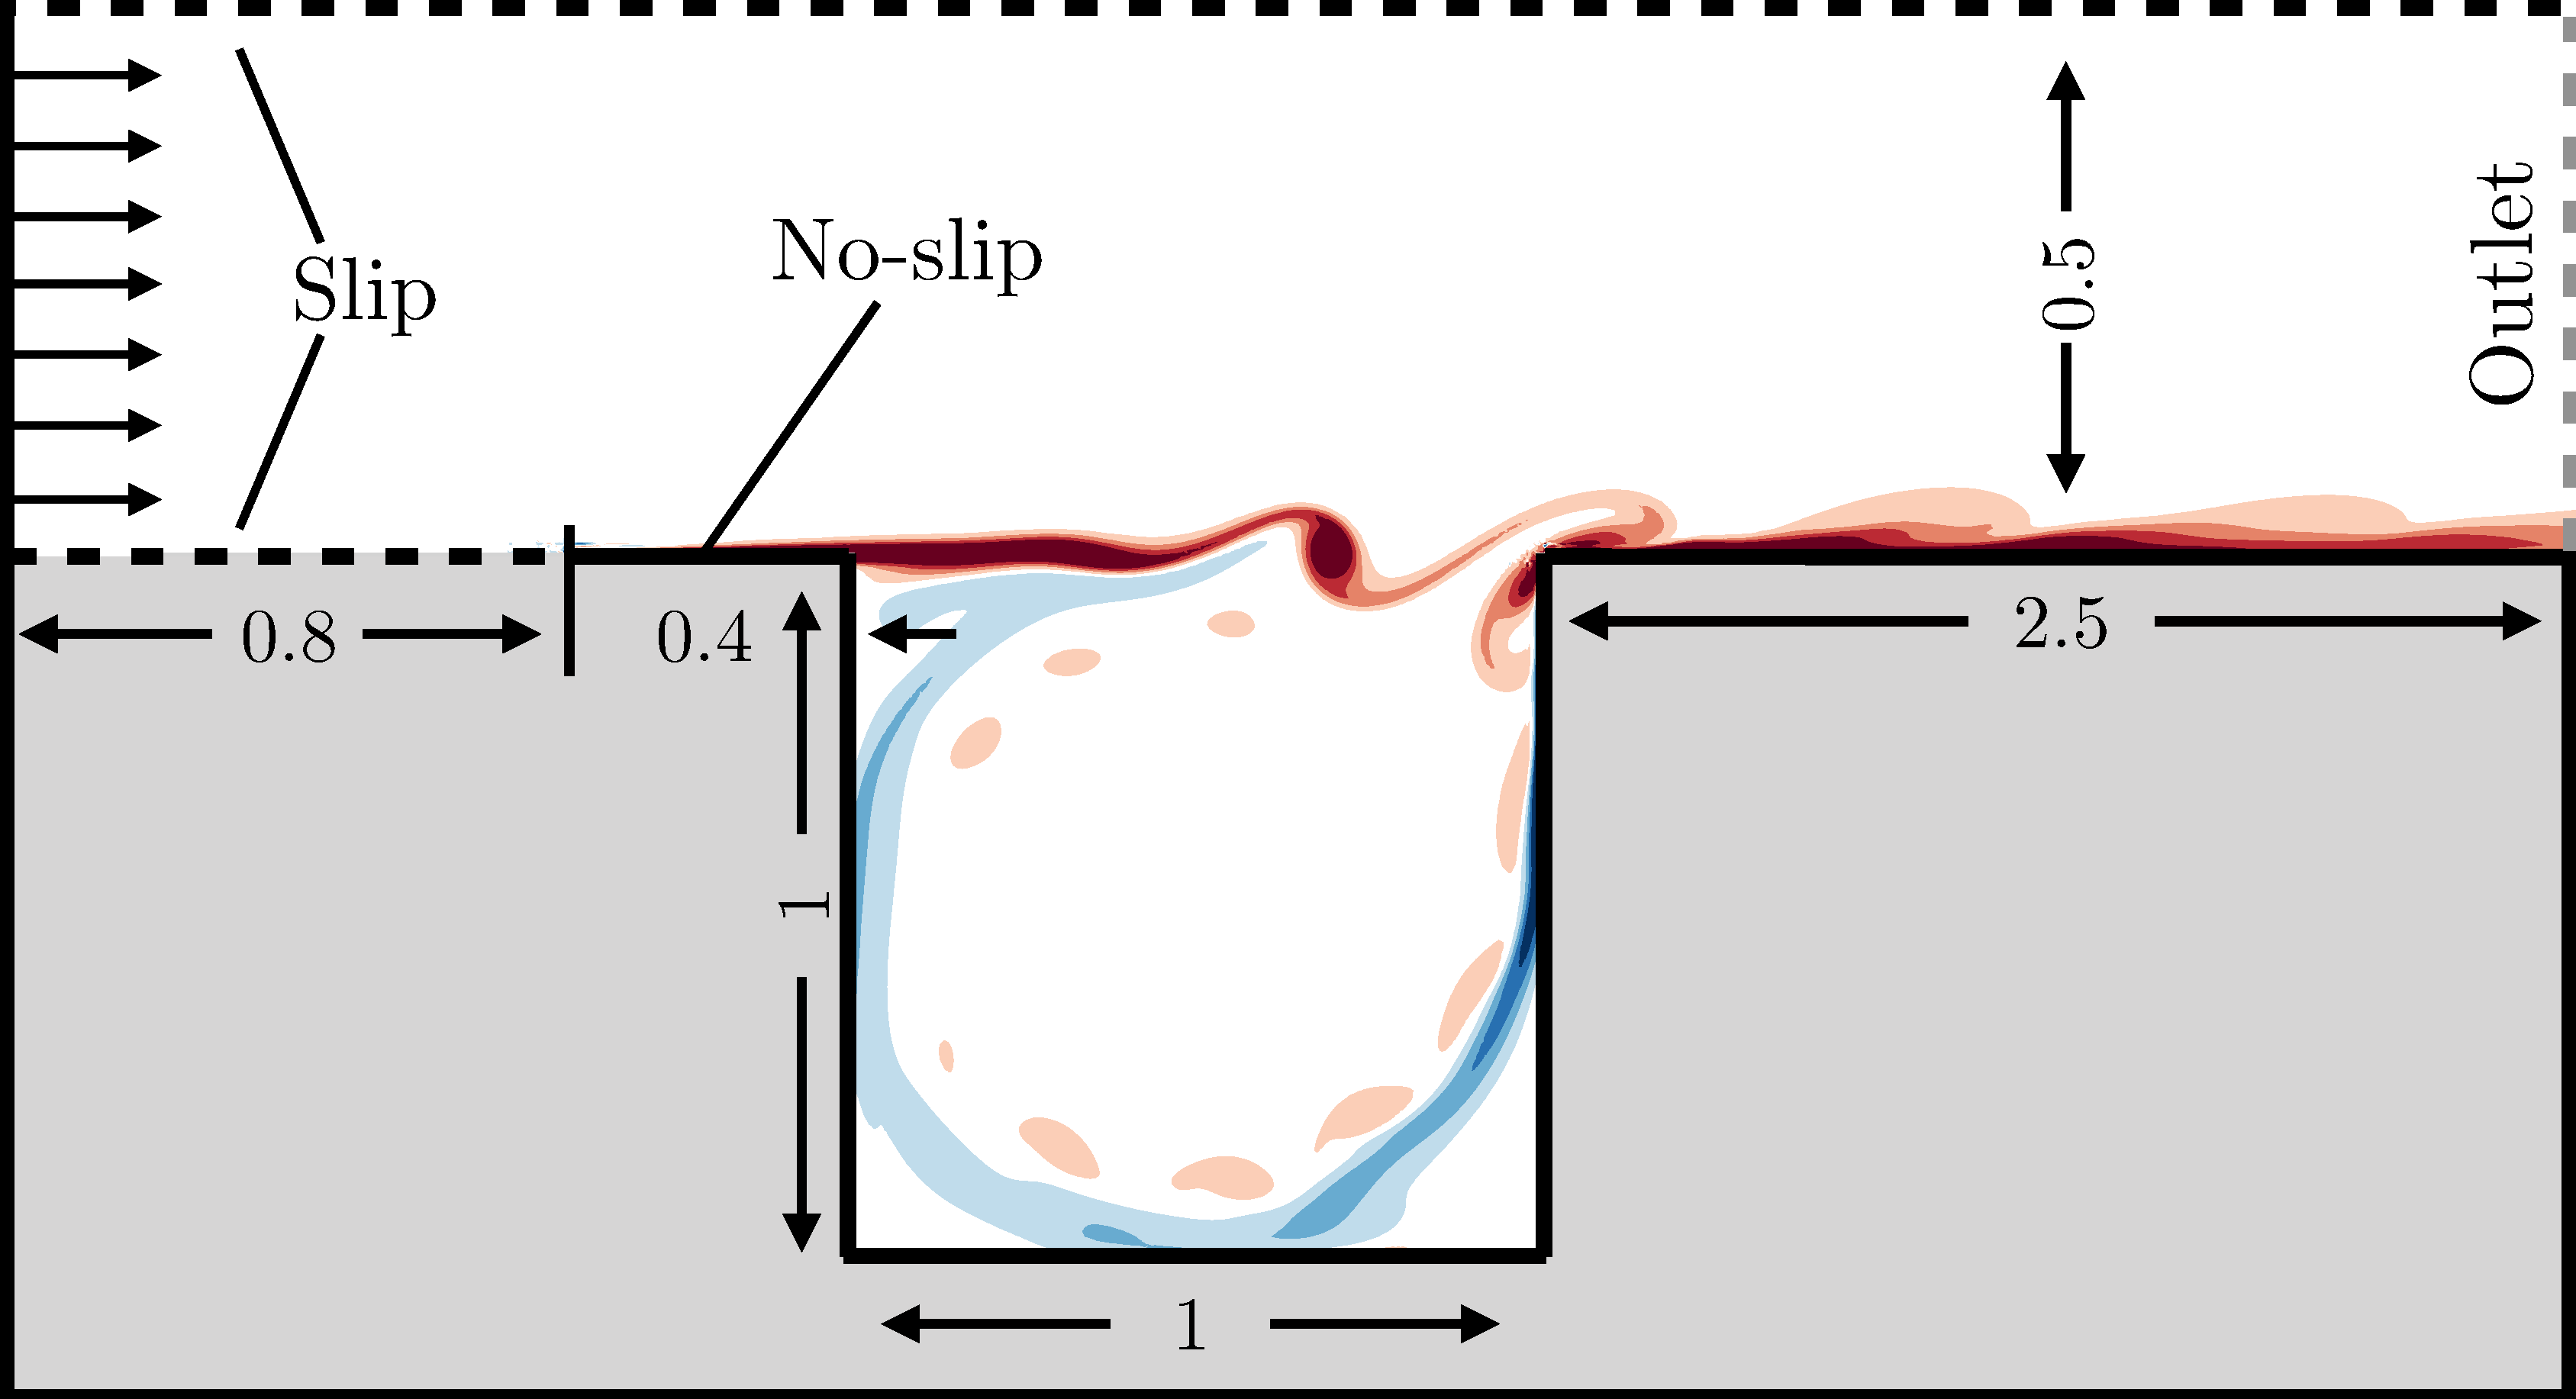
\includegraphics[width=\textwidth]{domain}
  \end{minipage}
  \vfill
\end{frame}


\begin{frame}
  \vfill
  \vfill
  \begin{minipage}{.28\textwidth}
    \centering
    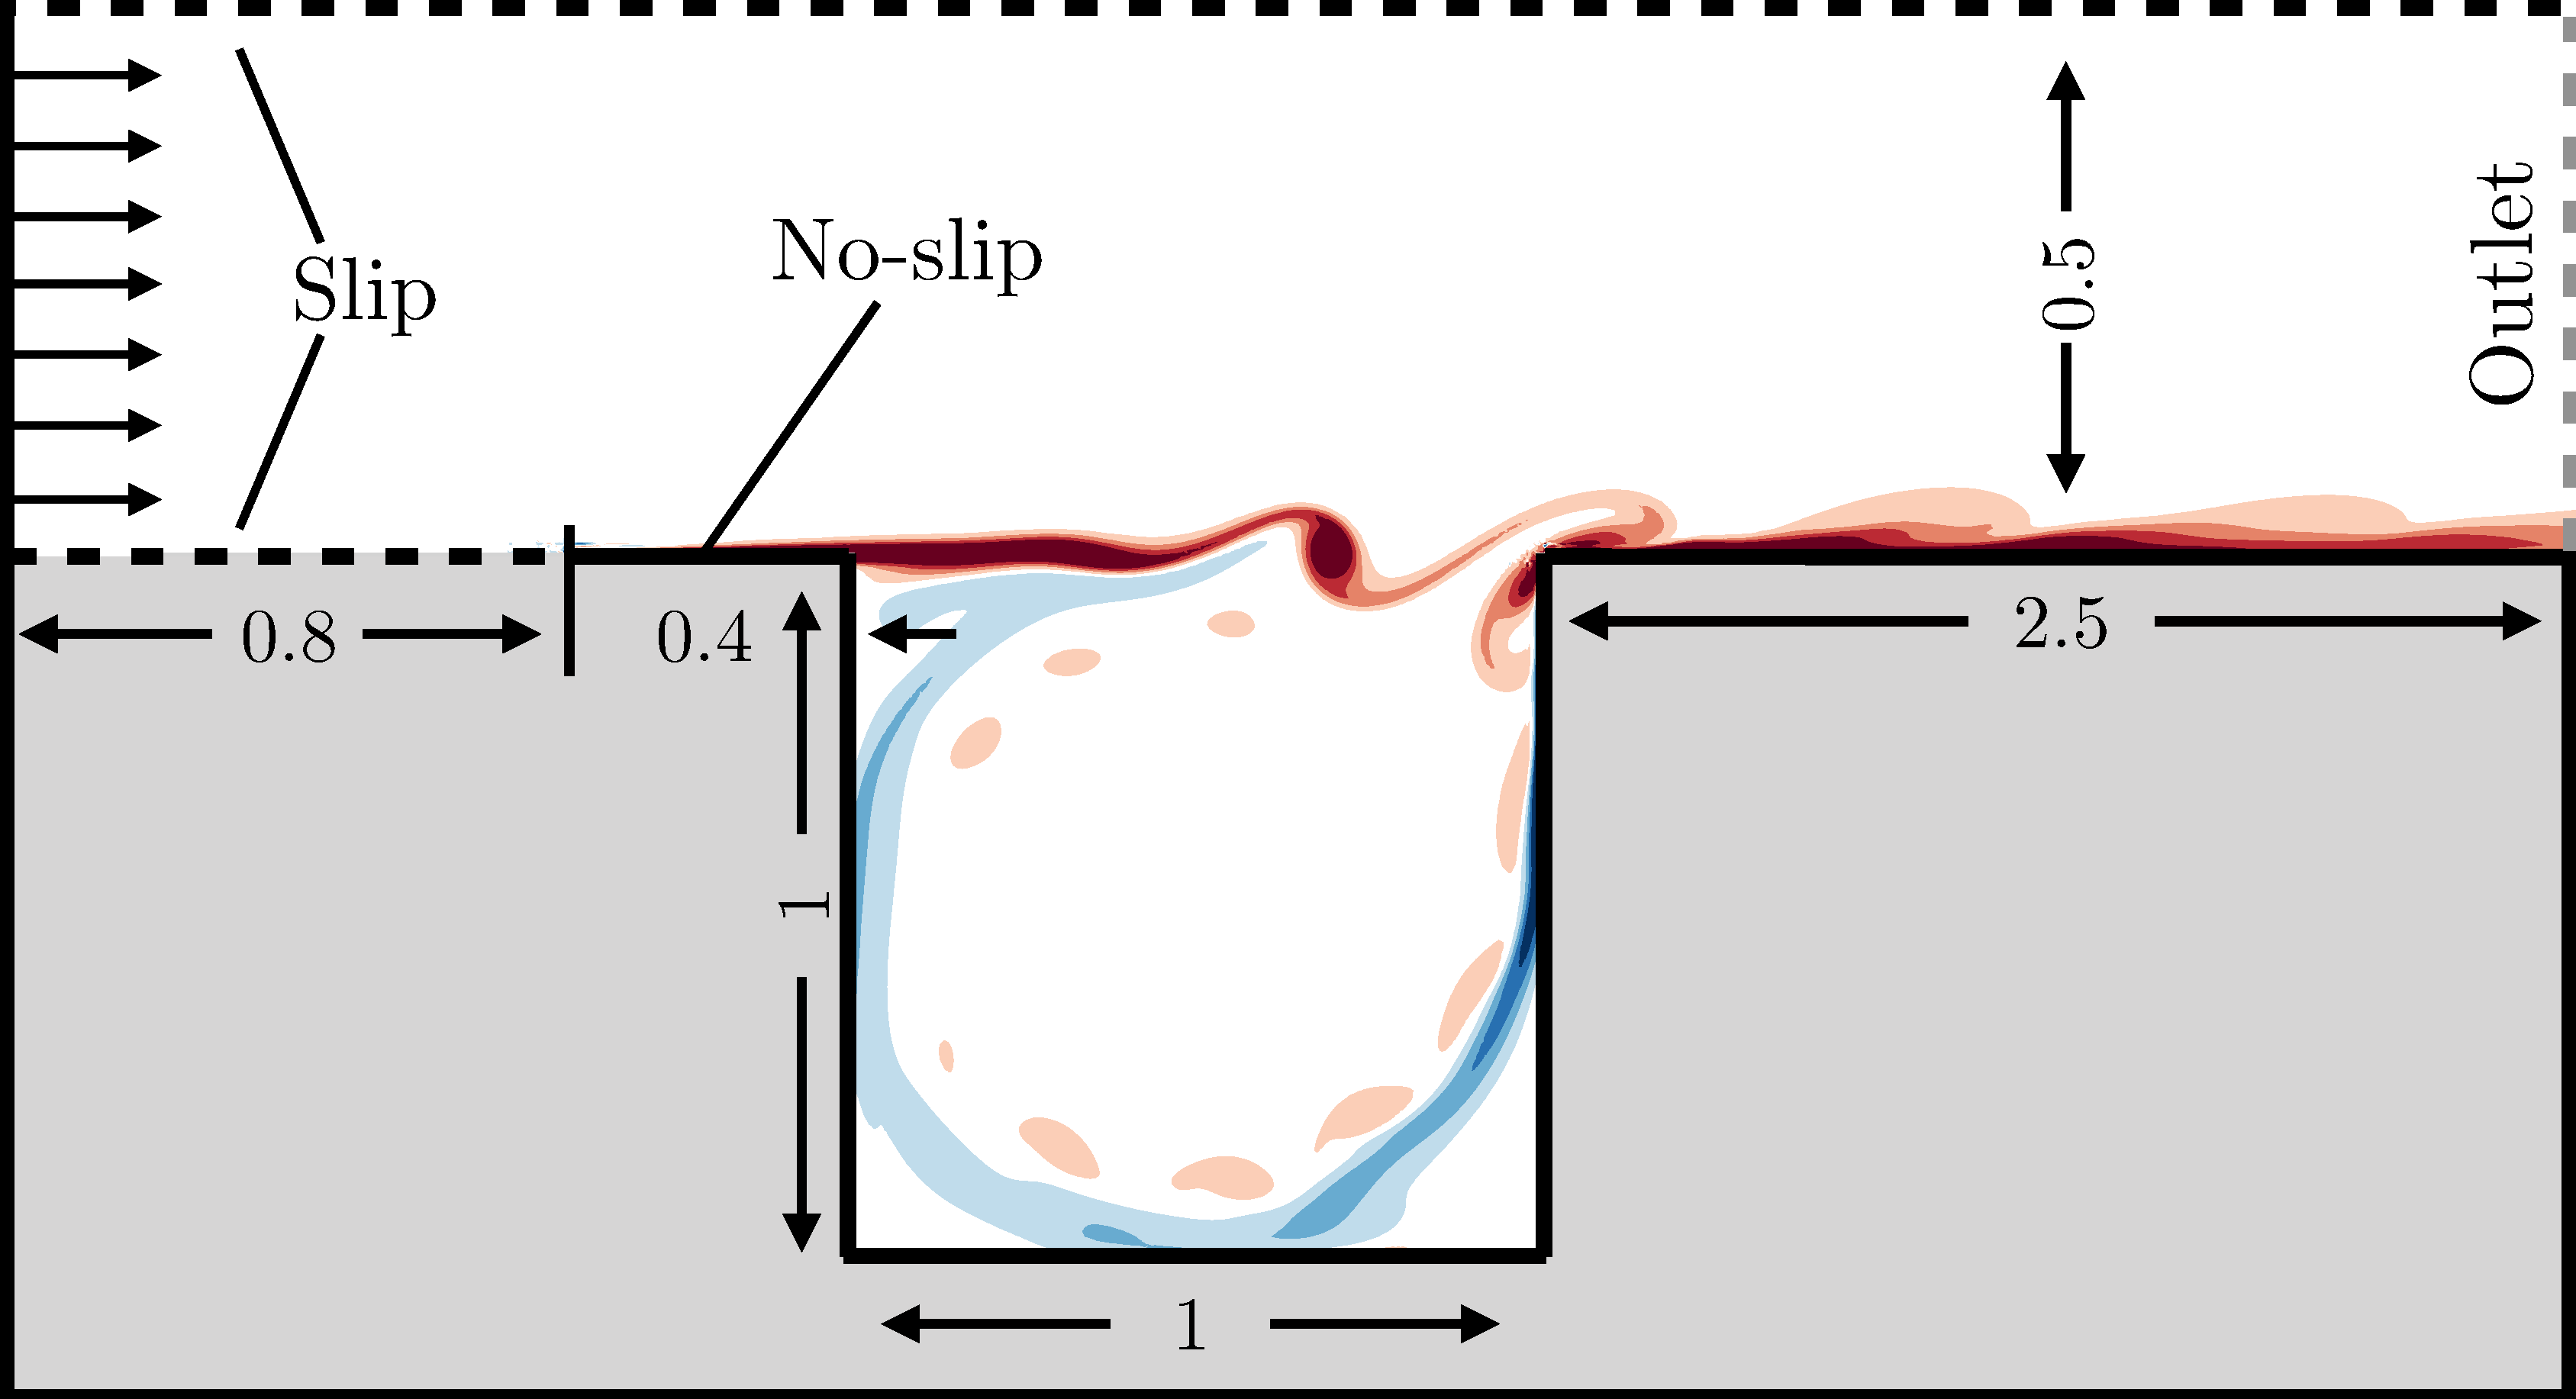
\includegraphics[width=\textwidth]{domain}
  \end{minipage}%
  \hfill
  \begin{minipage}{.68\textwidth}
    \begin{itemize}
    \item From $Re = 4000 \quad \to \quad Re = 4500$.\\
      \medskip
    \item 4000 spectral elements.
      \medskip
    \item 3\textsuperscript{rd} order-accurate EXT/BDF scheme.
      \medskip
    \item Helmholtz solver tolerance set to $10^{-12}$.
      \medskip
    \item Pressure Poisson solver tolerance set to $10^{-10}$.
    \end{itemize}
  \end{minipage}
  \vfill
\end{frame}


\begin{frame}
  \vfill
  \centering
  \textbf{Coarse mesh :} $64\ 000$ grid points with $\Delta t = 0.0025$

  \vfill
  
  \begin{tabular}{ccccc}
    ~ & \textbf{SFD} & \textbf{BootConv} & \textbf{Newton-GMRES} & \textbf{Newton-GMRES} (dyn. tol.) \\
    \\
    \hline \\
    \textbf{Time} & 975~\unit{\s} & 1600~\unit{\s} & 600~\unit{\s} & 400~\unit{\s}\\
    \\
    \textbf{RAM Usage} & 0.3~\unit{Gb} & 0.4~\unit{Gb} & 1.8~\unit{Gb} & 0.5~\unit{Gb} 
  \end{tabular}
  \vfill
\end{frame}


\begin{frame}
  \vfill
  \centering
  \textbf{Intermediate mesh :} $144\ 000$ grid points with $\Delta t = 0.001$

  \vfill
  
  \begin{tabular}{ccccc}
    ~ & \textbf{SFD} & \textbf{BootConv} & \textbf{Newton-GMRES} & \textbf{Newton-GMRES} (dyn. tol.) \\
    \\
    \hline \\
    \textbf{Time} & 3120~\unit{\s} & NA & 500~\unit{\s} & 400~\unit{\s}\\
      & ($\times 3.2$) &  & ($\times 1$) & ($\times 1$) \\
    \\
    \textbf{RAM Usage} & 0.4~\unit{Gb} &  & 1.8~\unit{Gb} & 0.8~\unit{Gb} 
  \end{tabular}
  \vfill
\end{frame}


\begin{frame}
  \vfill
  \centering
  \textbf{Fine mesh :} $256\ 000$ grid points with $\Delta t = 0.0006$

  \vfill
  
  \begin{tabular}{ccccc}
    ~ & \textbf{SFD} & \textbf{BootConv} & \textbf{Newton-GMRES} & \textbf{Newton-GMRES} (dyn. tol.) \\
    \\
    \hline \\
    \textbf{Time} & $10^4$~\unit{\s} & NA & 1900~\unit{\s} & 1500~\unit{\s}\\
      & ($\times 3.5$) &  & ($\times 3.8$) & ($\times 3.8$) \\
    \\
    \textbf{RAM Usage} & 0.6~\unit{Gb} &  & 2.9~\unit{Gb} & 0.8~\unit{Gb} 
  \end{tabular}
  \vfill
\end{frame}


}

\begin{frame}
  \vfill
  {
    \Large
    \[
      \begin{aligned}
        \exp\left( \tau \vb{L} \right) - \vb{I} & \simeq \left( \vb{I} + \tau \vb{L} \right) - \vb{I} \\
        & \propto \vb{L}
      \end{aligned}
    \]
  }
  \vfill
\end{frame}

\begin{frame}
  \vfill
  {
    \Large
    \[
      \mathrm{spec}(\vb{L}) \in \mathcal{D} = \left\{ z : \Re(z) \leq -\delta \right\}
    \]
  }
  \vfill
\end{frame}

\begin{frame}
  \vfill
  {
    \Large
    \[
      \mathrm{spec}(\vb{J}) \in \mathcal{D}^{\prime} = \left\{ z : \abs{z +1} \leq \exp(-\tau \delta) \right\}
    \]
  }
  \vfill
\end{frame}

\begin{frame}
  \vfill

  \centering
  The residual $\varepsilon$ after $k$ iterations can be upper bounded by

  {
    \Large
    \[
      \varepsilon \leq \kappa(\vb{V}) \exp(-k \tau \delta)
    \]
  }

  \bigskip
  
  with $\kappa(\vb{V})$ the condition number of the eigenbasis.

  \vfill
\end{frame}

\begin{frame}
  \vfill
  
  The number of iterations $k$ needed to reach a given tolerance $\varepsilon$ is given by

  {
    \Large
    \[
      k \leq \dfrac{1}{\tau \delta} \log \left( \dfrac{\kappa(\vb{V})}{\varepsilon} \right).
    \]
  }

  \bigskip

  This bound is however overly pessimistic. If $p$ eigenvalues are unstable, $\mathcal{O}(p)$ extra iterations are needed.
  
  \vfill
\end{frame}



\begin{frame}
  \vfill
  \begin{minipage}{.48\textwidth}
  \end{minipage}%
  \hfill
  \begin{minipage}{.48\textwidth}
    \centering
    {
      \huge
      \textbf{Linear stability analyses}
    }
  \end{minipage}
  \vfill
\end{frame}

\begin{frame}[t, c]{Spectral decomposition}{}
  \vfill
  \begin{minipage}{.48\textwidth}
    {
      \Large
      \[
        \exp \left( \tau \vb{L} \right) \vb{v} = \vb{v} \mu
      \]
    }
  \end{minipage}%
  \hfill
  \begin{minipage}{.48\textwidth}
    \begin{itemize}
    \item Matrix-vector product computed with a time-stepper.

      \bigskip

    \item Eigenvalues of interest already have the largest magnitude.

      \bigskip

    \item No other spectral transformation needed for fast convergence of iterative solvers.
    \end{itemize}
  \end{minipage}
  \vfill
\end{frame}

{
  \setbeamercolor*{background canvas}{bg=white}
  \setbeamercolor{normal text}{fg=black}
  \usebeamercolor[fg]{normal text}

  \begin{frame}
    \vfill
    \begin{minipage}{.28\textwidth}
    \end{minipage}%
    \hfill
    \begin{minipage}{.68\textwidth}
      \centering
      \textbf{Krylov subspace dimension :} 128
      
      \bigskip
      
      \begin{tabular}{rccc}
        \textbf{Mesh} & \emph{Coarse} & \emph{Intermediate} & \emph{Fine} \\
        \\
        \hline \\
        \textbf{\# of conv. ev.} & 2 & 2 & 2 \\
        \\
        \textbf{Time} & 30~\unit{\s} & 210~\unit{\s} & 800~\unit{\s}
      \end{tabular}
    \end{minipage}
    \vfill
  \end{frame}

  \begin{frame}
    \vfill
    \begin{minipage}{.28\textwidth}
    \end{minipage}%
    \hfill
    \begin{minipage}{.68\textwidth}
      \centering
      \textbf{Krylov subspace dimension :} 192
      
      \bigskip
      
      \begin{tabular}{rccc}
        \textbf{Mesh} & \emph{Coarse} & \emph{Intermediate} & \emph{Fine} \\
        \\
        \hline \\
        \textbf{\# of conv. ev.} & 4 & 10 & 10 \\
        \\
        \textbf{Time} & 54~\unit{\s} & 324~\unit{\s} & 1140~\unit{\s}
      \end{tabular}
    \end{minipage}
    \vfill
  \end{frame}

  \begin{frame}
    \vfill
    \begin{minipage}{.28\textwidth}
    \end{minipage}%
    \hfill
    \begin{minipage}{.68\textwidth}
      \centering
      \textbf{Krylov subspace dimension :} 256
      
      \bigskip
      
      \begin{tabular}{rccc}
        \textbf{Mesh} & \emph{Coarse} & \emph{Intermediate} & \emph{Fine} \\
        \\
        \hline \\
        \textbf{\# of conv. ev.} & 6 & 10 & 10 \\
        \\
        \textbf{Time} & 80~\unit{\s} & 418~\unit{\s} & 1520~\unit{\s}
      \end{tabular}
    \end{minipage}
    \vfill
  \end{frame}  
}

\begin{frame}
  \vfill
  Suppose $\mu_i$ is an isolated eigenvalue such that the rest of the spectrum is enclosed in the disk
  
  \bigskip
  
  {
    \Large
    \[
      \mathcal{D} = \left\{ z : \abs{z-c} < \rho \right\},
    \]
  }
  
  \bigskip
    
  \ie{} a disk centered in $c$ and of radius $\rho$.
  \vfill
\end{frame}

\begin{frame}
  \vfill

  Upper bound for the residual $\varepsilon_i$ associated to $\mu_i$ after a $k$-step Arnoldi factorization is given by

  {
    \Large
    \[
      \varepsilon_i \leq \kappa(\vb{V}) \left( \dfrac{\rho}{\abs{\mu_i - c}} \right)^k.
    \]
  }

  \bigskip
  
  The further apart $\mu_i$ is from the rest of the spectrum, the faster it converges.
  
  \vfill
\end{frame}

\begin{frame}
  \vfill
  \begin{itemize}
  \item The larger $\tau$, the larger the gap between $\mu_i$ and the rest of the spectrum.
    
    \bigskip
    
  \item The larger $\tau$, the fewer iterations are needed to converge the leading eigenspectrum.
    
    \bigskip
    
  \item The larger $\tau$, the more expensive each matrix-vector product is.
  \end{itemize}
  \vfill
\end{frame}

{
  \setbeamercolor*{background canvas}{bg=white}
  \setbeamercolor{normal text}{fg=black}
  \usebeamercolor[fg]{normal text}

  \begin{frame}
    \vfill
    \begin{minipage}{.48\textwidth}
      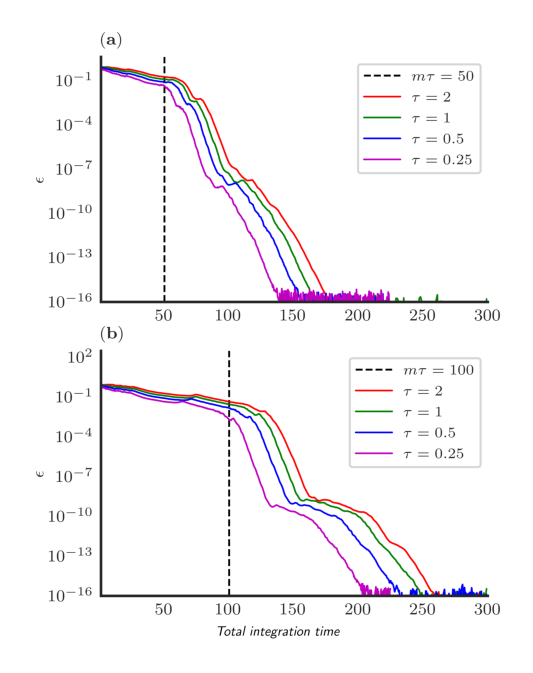
\includegraphics[width=\textwidth]{fig24}
    \end{minipage}%
    \hfill
    \begin{minipage}{.48\textwidth}
      For a random starting vector, the number of Krylov iterations before convergence is proportional to the flow-through time.
    \end{minipage}
    \vfill
  \end{frame}
}


\begin{frame}[t, c]{Adjoint sensitivity analysis}{}
  \vfill
  \begin{minipage}{.48\textwidth}
    \centering
    \textbf{Adjoint operator}
    
    \Large
    \[
      \langle \vb{y} \vert \vb{Lx} \rangle = \langle \vb{L}^{\dagger}\vb{y} \vert \vb{x} \rangle
    \]
  \end{minipage}%
  \hfill
  \begin{minipage}{.48\textwidth}
    \centering
    \textbf{Sensitivity to baseflow modification}
    
    \Large
    \[
      \nabla_{\vb{U}} \lambda = - \left( \nabla \vb{u} \right)^H \cdot \vb{u}^{\dagger} + \nabla \vb{u}^{\dagger} \cdot \vb{u}^*
    \]
  \end{minipage}
  \vfill
\end{frame}

\begin{frame}
  \vfill
  \centering
  \textbf{Sensitivity to a steady force}

  {
    \Large
    \[
      \nabla_{\vb{F}} \lambda = \vb{U}^{\dagger}
    \]

    \[
      \Updownarrow
    \]

    \[
      \vb{L}^{\dagger} \vb{U}^{\dagger} = \nabla_{\vb{U}} \lambda
    \]
  }
  \vfill
\end{frame}

\begin{frame}
  \vfill
  {
    \Large
    \[
      \dot{\vb{x}} = \vb{L}^{\dagger} \vb{x} + \vb{b}
    \]
  }
  \vfill
\end{frame}

\begin{frame}
  \vfill
  {
    \Large
    \[
      \vb{x}(\tau) = \exp(\tau \vb{L}^{\dagger}) \vb{x}_0 + \int_{0}^\tau \exp \left( (\tau - t) \vb{L}^{\dagger} \right) \vb{b} \ \dd t
    \]
  }
  \vfill
\end{frame}

\begin{frame}
  \vfill
  {
    \Large
    \[
      \left( \vb{I} - \exp(\tau \vb{L}^{\dagger}) \right) \vb{x} = \int_{0}^\tau \exp((\tau-t) \vb{L}^{\dagger}) \vb{b} \ \dd t
    \]
  }
  \vfill
\end{frame}

{
  \setbeamercolor*{background canvas}{bg=white}
  \setbeamercolor{normal text}{fg=black}
  \usebeamercolor[fg]{normal text}

  \begin{frame}
    \vfill
    \begin{minipage}{.48\textwidth}
      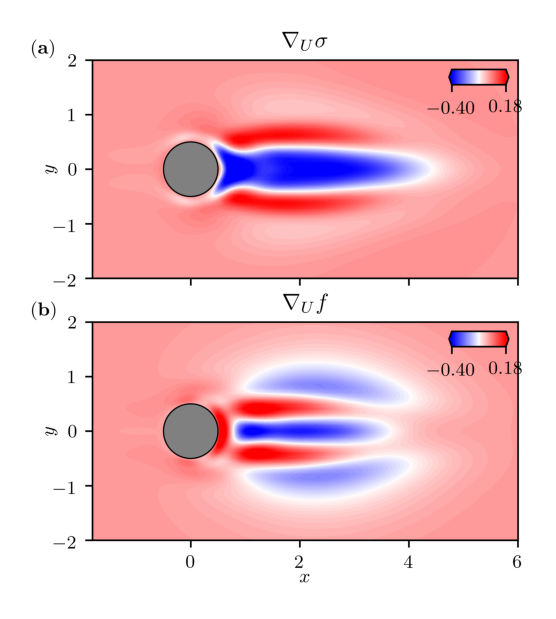
\includegraphics[width=\textwidth]{fig15}
    \end{minipage}%
    \hfill
    \begin{minipage}{.48\textwidth}
      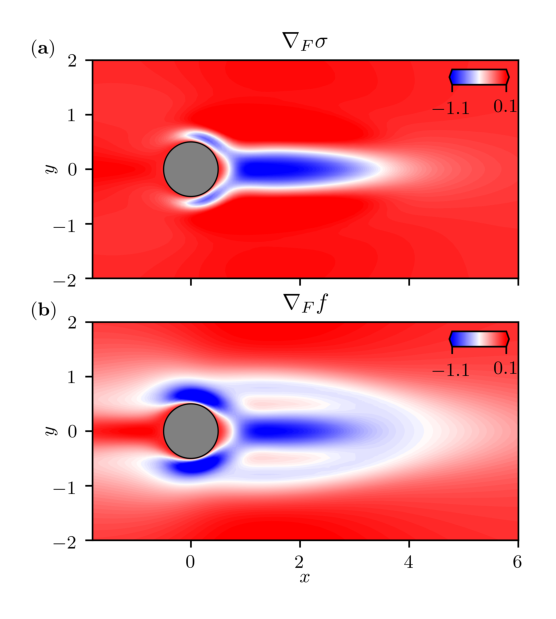
\includegraphics[width=\textwidth]{fig16}
    \end{minipage}
    \vfill
  \end{frame}
}


\begin{frame}
  \vfill
  \begin{minipage}{.48\textwidth}
  \end{minipage}%
  \hfill
  \begin{minipage}{.48\textwidth}
    \centering
    {
      \huge
      \textbf{What's next ?}
    }
  \end{minipage}
  \vfill
\end{frame}


\begin{frame}
  \vfill
  \begin{minipage}{.68\textwidth}
    \begin{itemize}
    \item Linear optimal perturbation analysis is a straightforward extension with the operator being
      %
      \[
        \vb{A} = \exp(\tau \vb{L}^{\dagger}) \exp(\tau \vb{L}).
      \]

      \medskip
      
    \item Resolvent analysis can also be cast in this framework although it requires being a bit more careful.
    \end{itemize}
  \end{minipage}%
  \hfill
  \begin{minipage}{.28\textwidth}
    \[
      \begin{aligned}
        \maximize_{\vb{x}} & \quad \norm{\exp(\tau \vb{L}) \vb{x}}_{\vb{W}}^2 \\
        \subto & \quad \norm{\vb{x}}_{\vb{W}}^2 = 1
      \end{aligned}
    \]
  \end{minipage}
  \vfill
\end{frame}

\begin{frame}
  \vfill
  \begin{itemize}
  \item Extension to compute (unstable) periodic orbits, satisfying
    %
    \[
      \vb{X} - \varphi_{\tau}(\vb{X}) = 0 \quad \text{for} \quad \tau = k \tau^*
    \]
    %
    is also straightforward.

    \bigskip

  \item The same applies to computing the eigenvalues of the monodromy matrix for Floquet analysis.
  \end{itemize}
  \vfill
\end{frame}


{
  \setbeamercolor*{background canvas}{bg=white}
  \setbeamercolor{normal text}{fg=black}
  \usebeamercolor[fg]{normal text}

  \begin{frame}
    \vfill
    \begin{minipage}{.28\textwidth}
      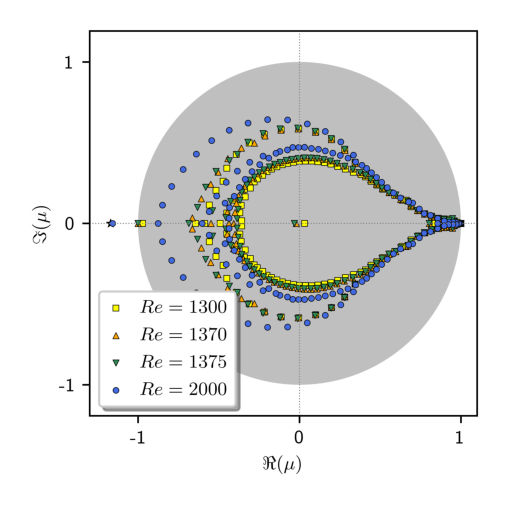
\includegraphics[width=\textwidth]{fig13}
    \end{minipage}%
    \hfill
    \begin{minipage}{.68\textwidth}
      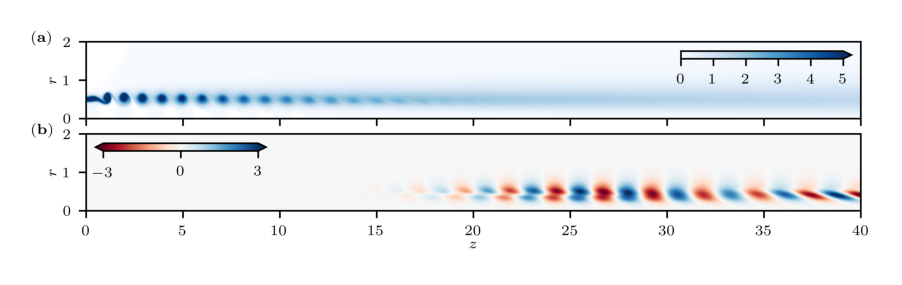
\includegraphics[width=\textwidth]{fig12}
    \end{minipage}
    \vfill
  \end{frame}

  \begin{frame}
    \vfill
    \centering
    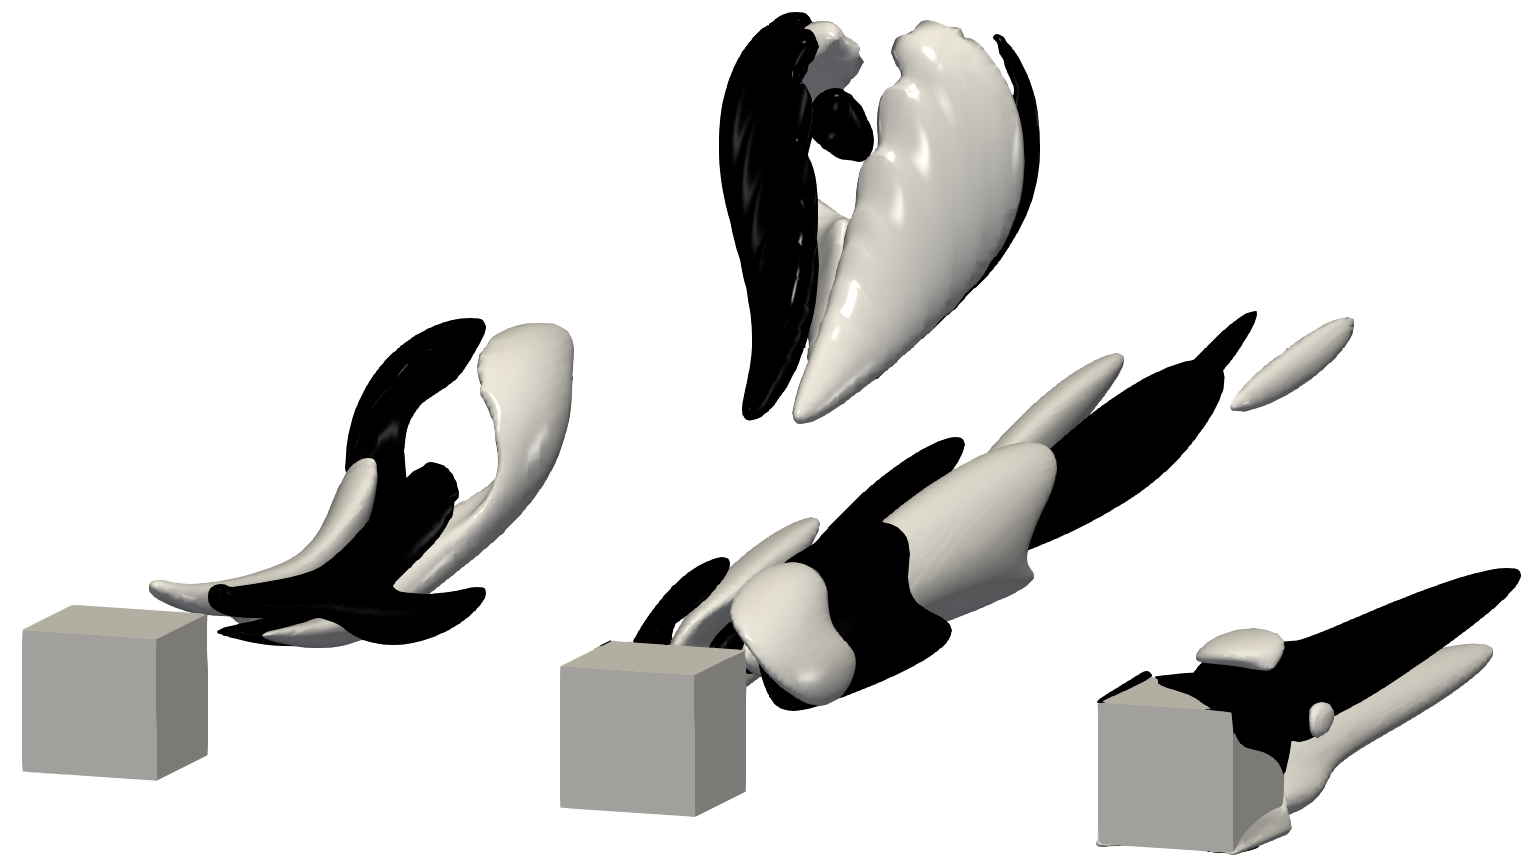
\includegraphics[width=.9\textwidth]{cube_bifurcations}
    \vfill
  \end{frame}
}

\begin{frame}
  \vfill
  \begin{minipage}{.68\textwidth}
    Quantitative comparison of the matrix-forming vs. time-stepper approaches using the exact same solver is still lacking.

    \bigskip

    If you have some extra \$\$\$ to use for this, please be my guest.
    You know how to get in touch with me !
  \end{minipage}%
  \hfill
  \begin{minipage}{.28\textwidth}
    \centering
    
\includegraphics[width=\textwidth]{question}
  \end{minipage}
  \vfill
\end{frame}
  
{
  \setbeamercolor*{background canvas}{bg=white}
  \setbeamercolor{normal text}{fg=black}
  \usebeamercolor[fg]{normal text}

  \begin{frame}
    \begin{minipage}{.28\textwidth}
      \centering
      
\includegraphics[height=.15\textheight]{github}
    \end{minipage}%
    \hfill
    \begin{minipage}{.68\textwidth}
      \url{https://loiseaujc.github.io/}
    \end{minipage}

    \bigskip

    \begin{minipage}{.28\textwidth}
      \centering
      
\includegraphics[width=\textwidth]{medium}
    \end{minipage}%
    \hfill
    \begin{minipage}{.68\textwidth}
      \url{https://loiseau-jc.medium.com/}
    \end{minipage}

    \bigskip

    \begin{minipage}{.28\textwidth}
      \centering
      
\includegraphics[height=.15\textheight]{twitter}
    \end{minipage}%
    \hfill
    \begin{minipage}{.68\textwidth}
      \url{@loiseau_jc}
    \end{minipage}

  \end{frame}
}

\begin{frame}
  \vfill
  \flushright

  {
  \Large
  \textbf{Thank you for your attention!}
  }

  \bigskip

  {
  \large
  \textcolor{gray}{
  \textbf{Any question?}
  }
  }
  \vfill
\end{frame}

\end{document}
